\documentclass[authoryear, 12pt]{elsarticle}

\usepackage{graphicx}
\usepackage{lineno}
\usepackage{amssymb}
\usepackage{wrapfig}
\usepackage{subfig}
\usepackage{tipa}
\usepackage{float}
\usepackage{longtable}
\usepackage[section]{placeins}
\usepackage{rotating}

\linespread{2}
\journal{}

\begin{document}

\begin{frontmatter}

\title{The development of children's ability to track and predict turn structure in conversation}

\author[MPI]{Marisa Casillas\corref{cor1}}
\address[MPI]{Max Planck Institute for Psycholinguistics, Nijmegen}
%\address[StanfordLX]{Department of Linguistics, Stanford University}
\cortext[cor1]{Corresponding author. \\ Address: Wundtlaan 1, 6525 XD, Nijmegen, The Netherlands\\ Email: marisa.casillas@mpi.nl \\Telephone: +31 024 3521 566; Fax: +31 024 3521 213}

\author[StanfordPSY]{Michael C. Frank}

\address[StanfordPSY]{Department of Psychology, Stanford University}

\begin{abstract}
Children begin developing turn-taking skills in infancy but take several years to assimilate their growing knowledge of language into their turn-taking behavior. In two eye-tracking experiments, we measured children's anticipatory gaze to upcoming responders while controlling linguistic cues to turn structure. In Experiment 1, we showed English and non-English conversations to English-speaking adults and children. In Experiment 2, we phonetically controlled lexicosyntactic and prosodic cues in English-only speech. Children spontaneously made anticipatory gaze switches by age two and continued improving through age six. In both experiments, children and adults made more anticipatory switches after hearing questions. Like adults, prosody alone did not improve children's predictive gaze shifts. But, unlike adults, lexical cues alone were not sufficient to improve prediction---children's performance was best overall with lexicosyntax and prosody together. Our findings support an account in which turn prediction emerges in infancy, but then only gradually becomes fully integrated with linguistic processing. 
\end{abstract}

\begin{keyword}
Turn taking \sep Conversation \sep Development \sep Questions \sep Eye-tracking \sep Anticipation
%% MSC codes here, in the form: \MSC code \sep code
%% or \MSC[2008] code \sep code (2000 is the default)

\end{keyword}

\end{frontmatter}

\linenumbers

\section{Introduction}
\label{sec:intro}

Spontaneous conversation is a universal context for using and learning language. Like other types of human interaction, it is organized at its core by the roles and goals of its participants. But, what sets conversation apart is its structure: sequences of interconnected, communicative actions that take place across alternating turns at talk. Sequential, turn-based structures in conversation are strikingly uniform across language communities and linguistic modalities. Turn-taking behaviors are also cross-culturally consistent in their basic features and the details of their implementation \citep{de-vos2015, dingemanse2013, stivers2009}. 

Children participate in sequential coordination (proto-turn taking) with their caregivers starting at three months of age---before they can rely on any linguistic cues \citep[see, among others, ][]{bateson1975, hilbrink2015, jaffe2001, snow1977}. However, infant turn taking is different from adult turn taking in several ways: it is heavily scaffolded by caregivers, has different timing from adult turn taking, and lacks semantic content \citep{hilbrink2015, jaffe2001}. But children's early, turn-structured social interactions are presumably a critical precursor to their later conversational turn taking. Early non-verbal interactions likely establish the protocol by which children come to use language with others. How do children integrate linguistic knowledge with these preverbal turn-taking abilities, and how does this integration change over the course of childhood? 

In this study, we investigate when children begin to make predictions about upcoming turn structure in conversation, and how they integrate language into their predictions as they grow older. In the remainder of the introduction, we first give a basic review of turn-taking research and the state of current knowledge about adult turn prediction. We then discuss recent work on the development of turn-taking skills before turning to the details of our own study.

\subsection{Adult turn taking}

Turn taking itself is not unique to conversation. Many other human activities are organized around sequential turns at action. Traffic intersections and computer network communication both use turn-taking systems. Children's early games (e.g., give-and-take, peek-a-boo) have built-in, predictable turn structure \citep{ratner1978, ross1987}. Even monkeys take turns: non-human primates such as marmosets and Campbell's monkeys vocalize contingently with each other in both natural and lab-controlled environments \citep{lemasson2011, takahashi2013}. In all these cases, turn taking serves as a protocol for interaction, allowing the participants to coordinate with each other through sequences of contingent action. 

Conversational turn taking distinguishes itself from other turn-taking behaviors by the complexity of the sequencing involved. Conversational turns come grouped into semantically-contingent sequences of action. The groups can span turn-by-turn exchanges (e.g., simple question--response, ``How are you?''--``Fine.'') or sequence-by-sequence exchanges (e.g., reciprocals, ``How are you?''--``Fine, and you?''--``Great!''). Compared to other turn-taking behaviors, the possible sequence and action types in everyday talk are can be diverse and unpredictable. 

% Sequences of action drive the conversation forward into the next, relevant sequences of talk (e.g., ''And you?''--``Great!''--``Why's that?''; \citealp{schegloff2007}). To take a turn, participants need to make predictions about what conversational content will be relevant next. In some cases, relevant next turns are somewhat obvious (e.g., question--response) while, in other cases, there are multiple relevant next actions to choose from or no obvious next action at all (e.g., after a closing).

Despite this complexity, conversational turn taking is precise in its timing. Across a diverse sample of conversations in 10 languages, one study found a consistent average turn transition time of 0--200 msec at points of speaker switch \citep{stivers2009}. Experimental results and current models of speech production suggest that it takes approximately 600 msec to produce a content word, and even longer to produce a simple utterance \citep{griffin2000, levelt1989}. So in order to achieve 200 msec turn transitions, speakers must begin formulating their response before the prior turn has ended \citep{levinson2013, levinson2016}. Moreover, to formulate their response early on, speakers must track and anticipate what types of response might become relevant next. They also need to predict the content and form of upcoming speech so that they can launch their articulation at exactly the right moment. Prediction thus plays a key role in timely turn taking.

Adults have a lot of information at their disposal to help make accurate predictions about upcoming turn content. Lexical, syntactic, and prosodic information (e.g., \textit{wh}- words, subject-auxiliary inversion, and list intonation) can all inform addressees about upcoming linguistic structure \citep{de-ruiter2006, duncan1972, ford1996, torreira2015}. Non-verbal cues (e.g., gaze, posture, and pointing) often appear at turn-boundaries and can sometimes act as late indicators of an upcoming speaker switch \citep{rossano2009, stivers2010}. Additionally, the sequential context of a turn can make it clear what will come next: answers after questions, thanks or denial after compliments, etc. \citep{schegloff2007}.

Prior work suggests that adult listeners primarily use lexicosyntactic information to accurately predict upcoming turn structure. De Ruiter and colleagues \citeyearpar{de-ruiter2006} asked participants to listen to snippets of spontaneous conversation and to press a button whenever they anticipated that the current speaker was about to finish his or her turn. The speech snippets were controlled for the amount of linguistic information present; some were normal, but others had flattened pitch, low-pass filtered speech, or further manipulations. With pitch-flattened speech, the timing of participants' button responses was comparable to their timing with the full linguistic signal. But when no lexical information was available, participants' responses were significantly earlier. The authors concluded that lexicosyntactic information\footnote{The ``lexicosyntactic'' condition only included flattened pitch and so was not exclusively lexicosyntactic---the speech would still have residual prosodic structure, including syllable duration and intensity.} was necessary and possibly sufficient for turn-end projection, while intonation was neither necessary nor sufficient. Congruent evidence comes from studies varying the predictability of lexicosyntactic and pragmatic content: adults anticipate turn ends better when they can more accurately predict the exact words that will come next (\citealp{magyari2012}; see also \citealp{magyari2014}). They can also identify speech acts within the first word of an utterance \citep{gisladottir2015}, allowing them to start planning their response at the first moment possible \citep{bogels2015}.

Despite this body of evidence, the role of prosody for adult turn prediction is still a matter of debate. De Ruiter and colleagues' (2006) experiment focused on the role of intonation, which is only a partial index of prosody. Prosody is tied closely to the syntax of an utterance, so the two linguistic signals are difficult to control independently \citep{ford1996}. \citet*{torreira2015} used a combination of button-press and verbal responses to investigate the relationship between lexicosyntactic and prosodic cues in turn-end prediction. Critically, their stimuli were cross-spliced so that each item had full prosodic cues to accompany the lexicosyntax. Because of the splicing, they were able to create items that had syntactically-complete units with no intonational phrase boundary at the end. Participants never verbally responded or pressed the ``turn-end'' button when hearing a syntactically-complete phrase without an intonational phrase boundary. And when intonational phrase boundaries were embedded in multi-utterance turns, participants were tricked into pressing the ``turn-end'' button 29\% of the time. Their results suggest that listeners actually do rely on prosodic cues to execute a response (see also de \citet{de-ruiter2006}:525). These experimental findings corroborate other corpus and experimental work promoting a combination of cues (lexicosyntactic, prosodic, and pragmatic) as key for accurate turn-end prediction \citep{duncan1972, ford1996, hirvenkari2013}. 

\subsection{Turn taking in development}

% Adults accurately and spontaneously make predictions about upcoming turn structure. Their predictions rely on a sophisticated body of knowledge about linguistic structure, non-verbal signals, and social actions. Knowing this, we could expect that children's acquisition of turn-taking skills is closely tied to their knowledge about language, gaze, gesture, and social cues. But children's turn taking starts early in infancy, long before their first words or gestures emerge. So a primary role for lexicosyntactic cues doesn't fit well with children's pre-verbal turn taking. 

The majority of work on children's early turn taking has focused on observations of spontaneous interaction. Children's first turn-like structures appear as early as two to three months after birth, in proto-conversation with their caregivers \citep{bruner1975, bruner1985}. During proto-conversations, caregivers treat their infants as capable of making meaningful contributions: they take every look, vocalization, arm flail, and burp as ``utterances'' in the joint discourse \citep{bateson1975, jaffe2001, snow1977}. Infants catch onto the structure of proto-conversations quickly. By three to four months they notice disturbances to the contingency of their caregivers' response and, in reaction, change the rate and quality of their vocalizations \citep{k-bloom1988, masataka1993, toda1993}. 

% Infants at this age also notice changes to social contingency outside of turn structure. In the Still Face paradigm, caregivers interact with their infants and then suddenly halt, taking on a neutral expression with a sustained gaze. When faced with this sudden disappearance of social contingency, infants three months and older try a range of methods to reinitiate the interaction, such as vocalization, reaching, and smiling before looking away or getting upset \citep{rochat1998, toda1993}.

The timing of children's responses to their caregivers' speech shows a non-linear pattern. Infants' contingent vocalizations in the first few months of life show very fast timing (though with a lot of vocal overlap). But by nine months, their timing slows down considerably, only to gradually speed up again after 12 months \citep{hilbrink2015}. For children, taking turns with brief transitions between speakers is more difficult than avoiding speaker overlap; children's incidence of overlap is nearly adult-like by nine months, but the timing of their non-overlapped responses stays much longer than the adult 200 msec standard for the next few years \citep{casillas2016, garvey1984, garvey1981, ervin-tripp1979}. This puzzling pattern is likely due to their linguistic development: taking turns on time is easier when the response is a simple vocalization rather than a linguistic utterance. Integrating language into the turn-taking system may therefore be one major factor in children's delayed responses \citep{casillas2016}.

Children, like adults, might use linguistic cues in the ongoing turn to make predictions about upcoming turn structure. Studies of early linguistic development point to a possible early advantage for prosody over lexicosyntax in children's turn-taking predictions. Infants can distinguish their native language's rhythm type from others soon after birth \citep{mehler1988, nazzi2003}; they show preference for the typical stress patterns of their native language over others by 6--9 months (e.g., iambic vs. trochaic), and can use prosodic information to segment the speech stream into smaller chunks from 8 months onward \citep{johnson2001, morgan1995}. Four- to five-month-olds also prefer pauses in speech to be inserted at prosodic boundaries, and by 6 months infants can use prosodic markers to pick out sub-clausal syntactic units, both of which are useful for extracting turn structure from ongoing speech \citep{jusczyk1995, soderstrom2003}. In comparison, children show at best a very limited lexical inventory before their first birthday \citep{bergelson2013, shi2010}.

%If response planning (i.e., language production) is the primary hurdle in young children's spontaneous turn taking, we should find evidence that children understand turn-taking behaviors before they are able to produce the behaviors themselves. This hypothesis has been recently explored in experimental settings, but results are mixed. One study found that 12-month-olds make more predictive gaze shifts to a responder while watching human verbal conversation compared to conversation-like interactions with objects \citep{bakker2011}, but another only found a similar effect at 36 months \citep{hofsten2009}. However, neither of these two studies had baselines to which the turn-relevant looking behavior could be compared. A baseline measurement is critical because there may be developmental differences in gaze shifting between conversational participants, even if the shifting is not related to turn structure. Such developmental differences could produce artifactual changes in measures of turn-contingent shifting. 

% Children begin to develop specific expectations about conversational behavior before they begin to speak. Sometime between four and six months, children begin to attend differently to face-to-face and back-to-back conversation; six-month-olds follow conversational speakers more with their gaze when at least one speaker is looking at the other \citep{augusti2010}. At ten months, infants expect people to look and talk at other people, and not to objects \citep{beier2012}. At twelve months infants expect to see responses to verbal (but not non-speech) utterances in face-to-face contexts \citep{thorgrimsson2015}.

% Prior work has focused mainly on lexicosyntax and intonation, and not on prosody proper (\citealp{de-ruiter2006}; \citealp{keitel2013}, but see \citealp{torreira2015}), even though infants seem to acquire the basic rhythmic properties of the prosodic signal first \citep{mehler1988, moon1993, nazzi2003}.

Keitel and colleagues \citeyearpar{keitel2013} were one of the first to explore how children use linguistic cues to predict upcoming turn structure. They asked 6-, 12-, 24-, and 36-month-old infants, and adult participants to watch short videos of conversation and tracked their eye movements at points of speaker change. They showed their participants two types of conversation videos---one normal and one with flattened pitch (i.e., with flattened intonation contours)---to test the role of intonation in participants' anticipatory predictions about upcoming speech. Comparing children's anticipatory gaze frequency to a random baseline, they found that only 36-month-olds and adults made anticipatory gaze switches more often than expected by chance. Among those, only 36-month-olds were affected by a lack of intonation contours, leading Keitel and colleagues to conclude that children's ability to predict upcoming turn structure relies on their ability to comprehend the stimuli lexicosemantically. They also suggest that intonation might play a secondary role in turn prediction, but only after children acquire more sophisticated, adult-like language comprehension abilities (also see \citealp{keitel2015}).

Although the Keitel et al. \citeyearpar{keitel2013} study constitutes a substantial advance over previous work in this domain, it has some limitations. Because these limitations directly inform our own study design, we review them in some detail. First, their estimates of baseline gaze frequency (``random'' in their terminology) were not random. Instead, they used gaze switches during ongoing speech as a baseline. But ongoing speech is the period in which switching is least likely to occur \citep{hirvenkari2013}---their baseline thus maximizes the chance of finding a difference in gaze frequency at turn transitions compared to the baseline. A more conservative baseline would compare participants' looking behavior at turn transitions to their looking behavior during randomly selected windows of time throughout the stimulus, including turn transitions. We follow this conservative approach in the current study. 

Second, the conversation stimuli \citet{keitel2013} used were somewhat unusual. The average gap between turns was 900 msec, a duration much longer than typical adult timing, which averages around 200 msec \citep{stivers2009}. The speakers in the videos were also asked to minimize their movements while performing scripted, adult-directed conversation, which would have created a somewhat unnatural interaction. Additionally, to produce more naturalistic conversation, it would have been ideal to localize the sound sources for the two voices in the video (i.e., to have the voices come out of separate left and right speakers). But both voices were recorded and played back on the same audio channel, which may have made it difficult to distinguish the two talkers. Again, we attempt to address these issues in our current study. Despite these minor methodological issues, the Keitel et al. \citeyearpar{keitel2013} study still demonstrates intriguing age-based differences in children's ability to predict upcoming turn structure. Our current work takes this paradigm as a starting point.\footnote{But also see \citet{casillas2012, casillas2013}.} 

\subsection{The current study}

Our goal in the current study is to find out when children begin to make predictions about upcoming turn structure and to understand how their predictions are affected by linguistic cues across development. We present two experiments in which we measured children's anticipatory gaze to responders while they watched conversation videos with natural (people speaking English vs. non-English; Experiment 1) and non-natural (puppets with phonetically manipulated speech; Experiment 2) control over the presence of lexical and prosodic cues. We tested children across a wide range of ages (Experiment 1: 3--5 years; Experiment 2: 1--6 years), with adult control participants in each experiment.

We highlight three primary findings: first, although children and adults use linguistic cues to make predictions about upcoming turn structure, they do so primarily in predict speaker transitions after questions (a speech act effect). This intriguing effect, which has not been reported previously, suggests that participants track unfolding speech for cues to upcoming speaker change, which may affect how they use linguistic cues more generally for anticipatory processing in conversation. Second, we find that children make more predictions than expected by chance starting at age two, but that this effect is small at first, and continues to improve through age six. Third, we find no evidence of an early prosody advantage in children's anticipations and, further, no evidence that prosodic or lexical cues alone can substitute for their combination in the full linguistic signal (as is proposed for adults; \citealp{de-ruiter2006}). Instead, anticipation is strongest for stimuli with the full range of cues. In sum, our findings support an account in which turn prediction emerges in infancy, but becomes fully integrated with linguistic processing only gradually across development.

\section{Experiment 1}
\label{sec:exp1}

We recorded participants' eye movements as they watched six short videos of two-person (dyadic) conversation interspersed with attention-getting filler videos. Each conversation video featured an improvised discourse in one of five languages (English, German, Hebrew, Japanese, and Korean). Participants saw two videos in English and one in every other language. The participants, all native English speakers, were only expected to understand the two videos in English. We showed participants non-English videos to limit their access to lexical information while maintaining their access to other cues to turn boundaries (e.g., (non-native) prosody, gaze, inbreaths, phrase final lengthening). Using this method, we compared children and adult's anticipatory looks from the current speaker to the upcoming speaker at points of turn transition in English and non-English videos.

\subsection{Methods}
\label{sec:methods1}

\subsubsection{Participants}

We recruited 74 children between ages 3;0--5;11 and 11 undergraduate adults to participate in the experiment. Our child sample included 19 three-year-olds, 32 four-year-olds, and 23 five-year-olds, all enrolled in a local nursery school. All participants were native English speakers. Approximately one-third (N=25) of the children's parents and teachers reported that their child regularly heard a second (and sometimes third or further) language, but only one child frequently heard a language that was used in our non-English video stimuli, and we excluded his data from analyses. None of the adult participants reported fluency in a second language.

\begin{figure}[t]
\begin{center}
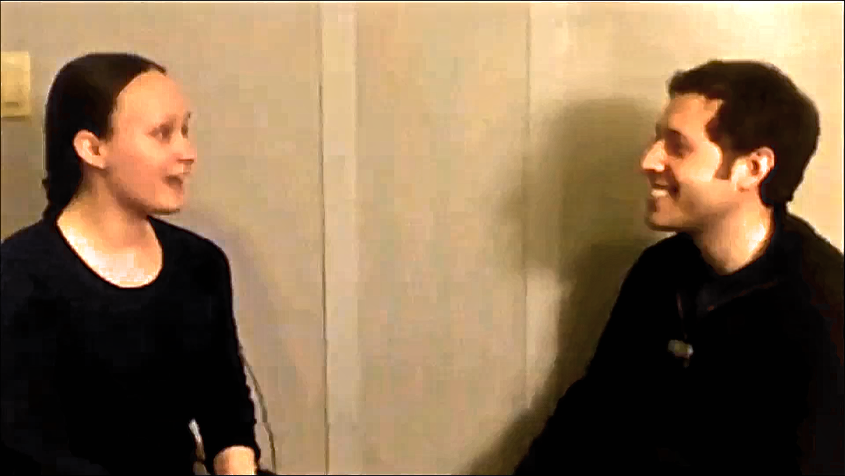
\includegraphics[width=0.6\textwidth]{figures/FIG-FL-stim.png}
\end{center}
\caption{Example frame from a conversation video used in Experiment 1.} 
\label{fig:speakers}
\end{figure}

\subsubsection{Materials}

\textit{Video recordings}. We recorded pairs of talkers while they conversed in a sound-attenuated booth (see a sample frame in Figure \ref{fig:speakers}). Each talker was a native speaker of the language being recorded, and each talker pair was male-female. Using a Marantz PMD 660 solid state field recorder, we captured audio from two lapel microphones, one attached to each participant, while simultaneously recording video from the built-in camera of a MacBook laptop computer. The talkers were volunteers and were acquainted with their recording partner ahead of time. 

Each recording session began with a 20-minute warm-up period of spontaneous conversation during which the pair talked for five minutes on four topics (favorite foods, entertainment, hometown layout, and pets). Then we asked talkers to choose a new topic---one relevant to young children (e.g., riding a bike, eating breakfast)---and to improvise a dialogue on that topic. We asked them to speak as if they were on a children's television show in order to elicit child-directed speech toward each other. We recorded until the talkers achieved at least 30 seconds of uninterrupted discourse with enthusiastic, child-directed speech. Most talker pairs took less than five minutes to complete the task, usually by agreeing on a rough script at the start. We encouraged talkers to ask at least a few questions to each other during the improvisation. The resulting conversations were therefore not entirely spontaneous, but were as close as possible while still remaining child-oriented in topic, prosodic pattern, and lexicosyntactic construction.\footnote{All of the non-English talkers were fluent in English as a second language, and some fluently spoke three or more languages. We chose male-female pairs as a natural way of creating contrast between the two talker voices.}

After recording, we combined the audio and video recordings by hand, and cropped each recording to the (approximate) 30-second interval with the most turn activity. Because we recorded the conversations in stereo, the male and female voices came out of separate speakers during video playback. This gave each voice in the videos a localized source (from the left or right loudspeaker). We coded each turn transition in the videos for language condition (English vs. non-English), inter-turn gap duration (in milliseconds), and speech act (question vs. non-question). The non-English stimuli were coded for speech act from a monolingual English-speaker's perspective, i.e., which turns ``sound like'' questions, and which do not: we asked five native American English speakers to listen to the audio recording for each non-English turn and judge whether it sounded like a question. We marked non-English turns as questions when at least 4 of the 5 listeners (80\%) said that the turn ``sounded like a question''.

Because the conversational stimuli were recorded semi-spontaneously, the duration of turn transitions and the number of speaker transitions in each video was variable. We measured the duration of each turn transition from the audio recording associated with each video. We excluded turn transitions longer than 550 msec and shorter than 90 msec, also excluding overlapped transitions, from analysis.\footnote{Overlap occurs when a responder begins a new turn before the current turn is finished. When overlap occurs, observers cannot switch their gaze in anticipation of the response because the response began earlier than expected. Participants expect conversations to proceed with ``one speaker at a time'' \citep{sacks1974}. They would therefore still be fixated on the prior speaker when the overlap started, and would have to switch their gaze \textit{reactively} to the responder.} This left approximately equal numbers of turn transitions available for analysis in the English (N$=$20) and non-English (N$=$16) videos. On average, the inter-turn gaps for English videos (mean$=$318, median$=$302, stdev$=$112 msec) were slightly longer than for non-English videos (mean$=$286, median$=$251, stdev$=$122 msec). The longer gaps in the English videos could give them a slight advantage: our definition of an ``anticipatory gaze shift'' includes shifts that are initiated during the gap between turns (Figure \ref{fig:criterion}), so participants had slightly more time to make anticipatory shifts in the English videos.

Questions made up exactly half of the turn transitions in the English (N$=$10) and non-English (N$=$8) videos. In the English videos, inter-turn gaps were slightly shorter for questions (mean$=$310, median$=$293, stdev$=$112 msec) than non-questions (mean$=$325, median$=$315, stdev$=$118 msec). Non-English videos did not show a large difference in transition time for questions (mean$=$270, median$=$257, stdev$=$116 msec) and non-questions (mean$=$302, median$=$252, stdev$=$134 msec).

\subsubsection{Procedure} 
Participants sat in front of an SMI 120Hz corneal reflection eye-tracker mounted beneath a large flatscreen display. The display and eye-tracker were secured to a table with an ergonomic arm that allowed the experimenter to position the whole apparatus at a comfortable height, approximately 60 cm from the viewer. We placed stereo speakers on the table, to the left and right of the display. 

Before the experiment started, we warned adult participants that they would see videos in several languages and that, though they weren't expected to understand the content of non-English videos, we \textit{would} ask them to answer general, non-language-based questions about the conversations. Then after each video we asked participants one of the following randomly-assigned questions: ``Which speaker talked more?'', ``Which speaker asked the most questions?'', ``Which speaker seemed more friendly?'', and ``Did the speakers' level of enthusiasm shift during the conversation?'' We also asked if the participants could understand any of what was said after each video. The participants responded verbally while an experimenter noted their responses.

Children were less inclined to simply sit and watch videos of conversation in languages they didn't speak, so we used a different procedure to keep them engaged: the experimenter started each session by asking the child about what languages he or she could speak, and about what other languages he or she had heard of. Then the experimenter expressed her own enthusiasm for learning about new languages, and invited the child to watch a video about ``new and different languages'' together. If the child agreed to watch, the experimenter and the child sat together in front of the display, with the child centered in front of the tracker and the experimenter off to the side. Each conversation video was preceded and followed by a 15--30 second attention-getting filler video (e.g., running puppies, singing muppets, flying bugs). If the child began to look bored, the experimenter would talk during the fillers, either commenting on the previous conversation (``That was a neat language!'') or giving the language name for the next conversation (``This next one is called Hebrew. Let's see what it's like.'') The experimenter's comments reinforced the video-watching as a joint task.

All participants (child and adult) completed a five-point calibration routine before the first video started. We used a dancing Elmo for the children's calibration image. During the experiment, participants watched all six 30-second conversation videos. The first and last conversations were in American English and the intervening conversations were Hebrew, Japanese, German, and Korean. The presentation order of the non-English videos was shuffled into four lists, which participants were assigned to randomly. The entire experiment, including instructions, took 10--15 minutes.

\subsubsection{Data preparation and coding}
\label{sec:algorithm}

To determine whether participants predicted upcoming turn transitions, we needed to define a set of criteria for what counted as an anticipatory gaze shift. Prior work using similar experimental procedures has found that adults and children make anticipatory gaze shifts to upcoming talkers within a wide time frame; the earliest shifts occur before the end of the prior turn, and the latest occur after the onset of the response turn, with most shifts occurring in the inter-turn gap (Keitel et al., 2013; Hirvenkari, 2013; Tice and Henetz, \citeyear{TiceHenetz11}). Following prior work, we measured how often our participants shifted their gaze from the prior to the upcoming speaker \textit{before} the shift in gaze could have been initiated in reaction to the onset of the speaker's response. In doing so, we assumed that it takes participants 200 msec to plan an eye movement, following standards from adult anticipatory processing studies \citep[e.g., ][]{kamide2003}.

We checked each participant's gaze at each turn transition for three characteristics (Figure \ref{fig:criterion}): (1) that the participant fixated on the prior speaker for at least 100 msec at the end of the prior turn, (2) that sometime thereafter the participant switched to fixate on the upcoming speaker for at least 100 ms, and (3) that the switch in gaze was initiated within the first 200 msec of the response turn, or earlier. These criteria guarantee that we only counted gaze shifts when: (1) participants were tracking the previous speaker, (2) switched their gaze to track the upcoming speaker, and (3) did so before they could have simply reacted to the onset of speech in the response. Under this assumption, a gaze shift that was initiated within the first 200 msec of the response (or earlier) was planned \textit{before} the child could react to the onset of speech itself. 

As mentioned, most anticipatory switches happen in the inter-turn gap, but we also allowed anticipatory gaze switches that occurred in the final syllables of the prior turn. Early switches are consistent with the distribution of responses in explicit turn-boundary prediction tasks. For example, in a button press task, adult participants anticipate turn ends approximately 200 msec in advance of the turn's end, and anticipatory responses to pitch-flattened stimuli come even earlier \citep{de-ruiter2006}. We therefore allowed switches to occur as early as 200 msec before the end of the prior turn. Again, because it takes 200 msec to plan an eye movement, we counted anticipatory switches, at the latest, 200 msec after the onset of speech. Therefore, for very early and very late switches, our requirement of 100 msec of fixation on each speaker would sometimes extend outside of the transition window boundaries (200 msec before and after the inter-turn gap). The maximally available fixation window was therefore 100 msec before and after the earliest and latest possible switch point (300 msec before and after the inter-turn gap). We did not count switches made during the fixation window as anticipatory. We \textit{did} count switches made during the inter-turn gap. The period of time from the beginning of the possible fixation window on the prior speaker to the end of the possible fixation window on the responder was our total analysis window (300 msec $+$ the inter-turn gap $+$ 300 msec).

\begin{figure}[t]
\begin{center}
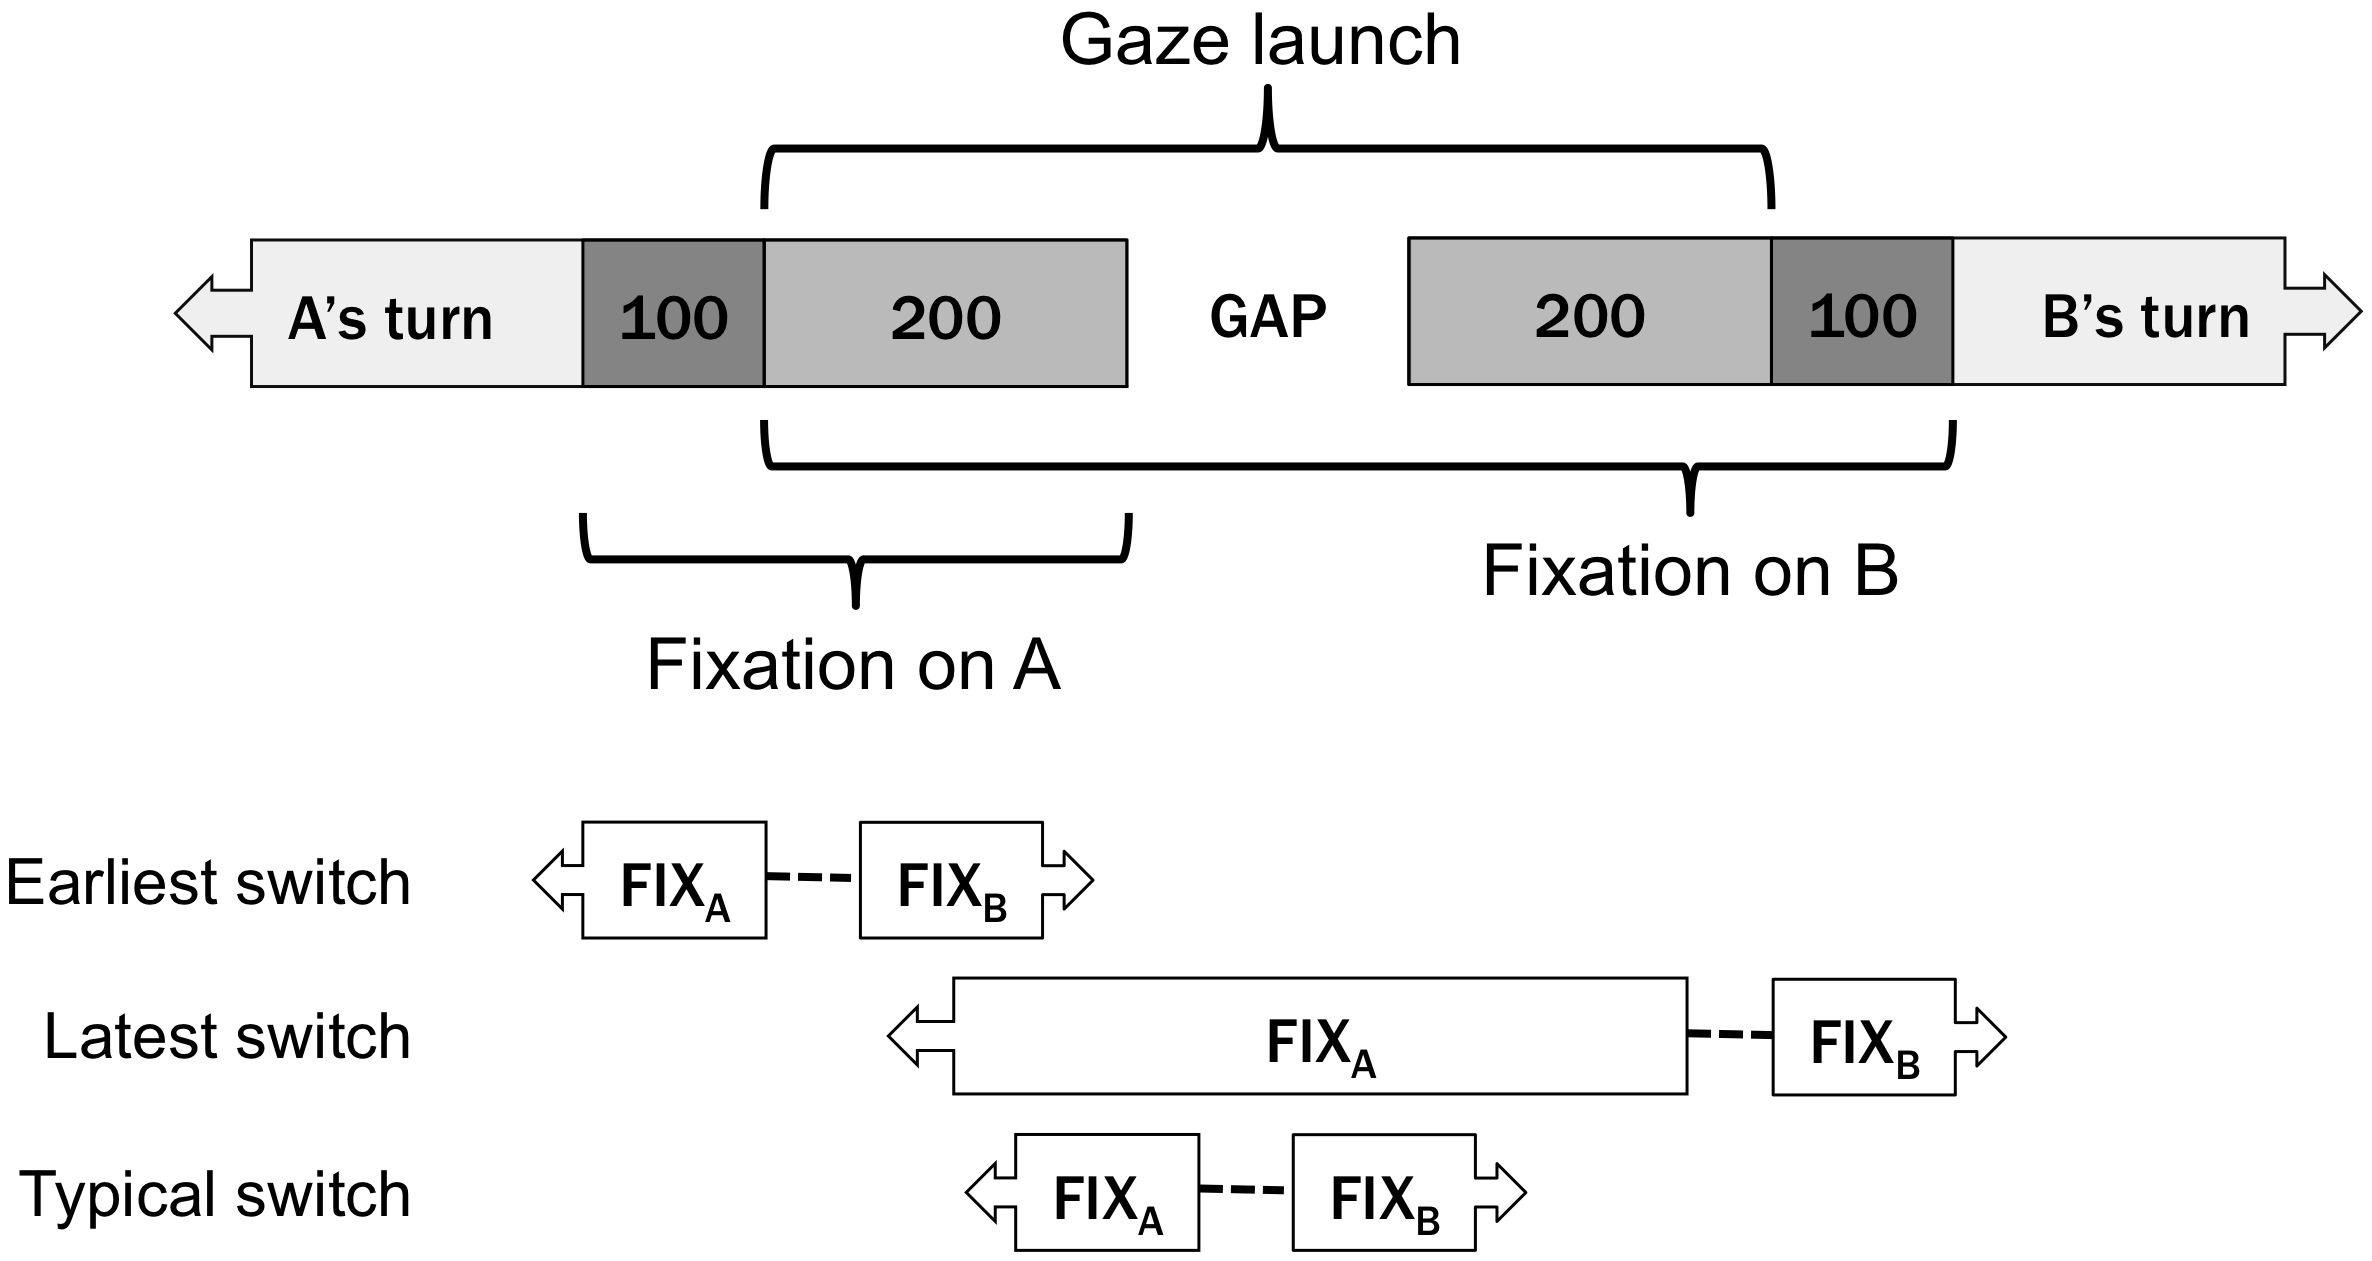
\includegraphics[width=0.7\textwidth]{figures/FIG-AnticipCriteria.png}
\end{center}
\caption{Schematic summary of criteria for anticipatory gaze shifts from speaker A to speaker B during a turn transition.} 
\label{fig:criterion}
\end{figure}

\paragraph{Predictions}
We expected participants to show greater anticipation in the English videos than in the non-English videos because of their increased access to linguistic information in English. We also predicted that anticipation would be greater following questions compared to non-questions; questions have early cues to upcoming turn transition (e.g., \textit{wh-} words, subject-auxiliary inversion), and also make a next response immediately relevant. Our third prediction was that anticipatory looks would increase with development, along with children's increased linguistic competence.

\subsection{Results}
\label{sec:results1}

Participants looked at the screen most of the time during video playback (81\% and 91\% on average for children and adults, respectively). They primarily kept their eyes on the person who was currently speaking in both English and non-English videos: they gazed at the current speaker between 38\% and 63\% of the time, looking back at the addressee between 15\% and 20\% of the time (Table \ref{tab:e1_look}). Even three-year-olds looked more at the current speaker than anything else, whether the videos were in a language they could understand or not. Children looked at the current speaker less than adults did during the non-English videos. Despite this, their looks to the addressee did not increase substantially in the non-English videos, indicating that their looks away were probably related to boredom rather than confusion about ongoing turn structure. Overall, participants' pattern of gaze to current speakers demonstrated that they performed basic turn tracking during the videos, regardless of language. Figure \ref{fig:E1-randvsreal} shows participants' anticipatory gaze rates across age, language condition, and transition type.

\linespread{1}
\begin{table}[t]
\begin{center}
  \begin{tabular}{llcccc}
    \hline
    Age group & Condition & Speaker & Addressee & Other onscreen & Offscreen\\ 
    \hline
    3 & English & 0.61 & 0.16 & 0.14 & 0.08 \\ 
    4 & English & 0.60 & 0.15 & 0.11 & 0.13 \\ 
    5 & English & 0.57 & 0.15 & 0.16 & 0.12 \\ 
    Adult & English & 0.63 & 0.16 & 0.16 & 0.05 \\ 
    3 & Non-English & 0.38 & 0.17 & 0.20 & 0.25 \\ 
    4 & Non-English & 0.43 & 0.19 & 0.21 & 0.18 \\ 
    5 & Non-English & 0.40 & 0.16 & 0.26 & 0.18 \\ 
    Adult & Non-English & 0.58 & 0.20 & 0.16 & 0.07 \\ 
%   Overall & & 0.49 & 0.17 & 0.18 & 0.16 \\
    \hline
  \end{tabular}
\end{center}
  \caption{Average proportion of gaze to the current speaker and addressee during periods of talk.}
\label{tab:e1_look}
\end{table}
\linespread{2}

\begin{figure}[h]
\begin{center}
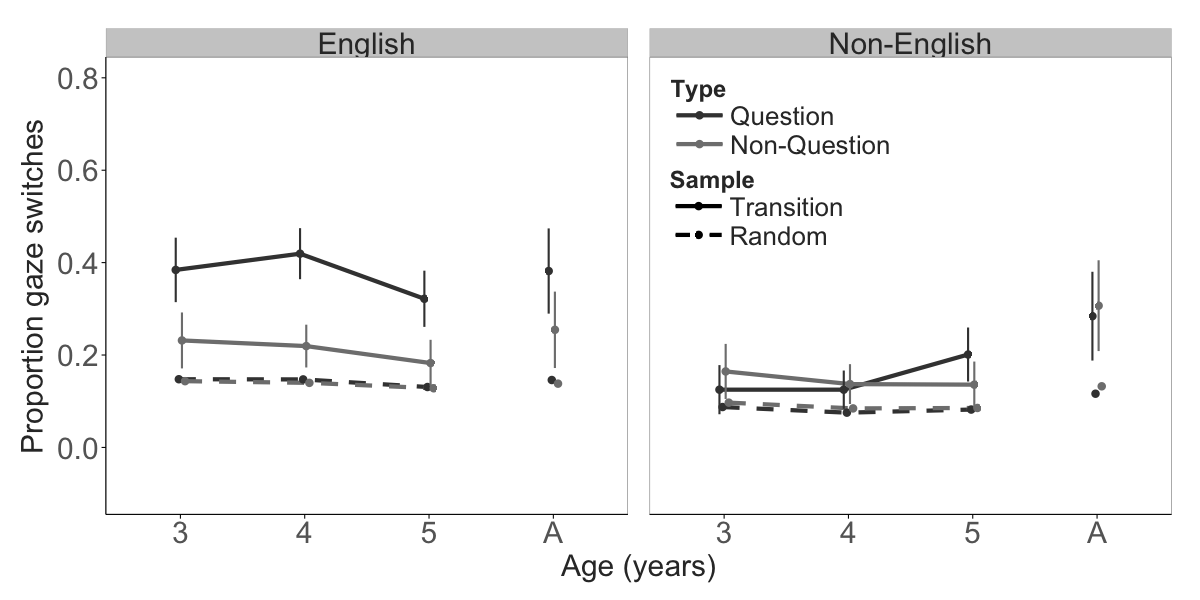
\includegraphics[width=1\textwidth]{figures/E1-samples-by-lang-groups-trans-types.png}
\end{center}
\caption{Anticipatory gaze rates across language condition and transition type for the real data (red and blue) and the randomly permuted baselines (gray). Vertical bars represent 95\% confidence intervals.} 
\label{fig:E1-randvsreal}
\end{figure}

\linespread{1}
\begin{table}[h!]
\begin{small}
\begin{center}
  \begin{tabular}{lcccl}
  \textbf{\textit{Children}} &&&& \\
    \hline
			           &  Estimate & Std. Error & \textit{z} value & Pr($>$$|$\textit{z}$|$) \\    
    \hline
    (Intercept)   										& -0.96145	& 0.84915		& -1.132	& 0.257531 	\\    
    Age             										& -0.18268	& 0.17509		& -1.043	& 0.296764   	\\  
    LgCond$=$\textit{non-English} 			& -3.29349	& 0.96055		& -3.429	& 0.000606 *** 	\\
    Type$=$\textit{non-Question}      	& -1.10131	& 0.86520		& -1.273	& 0.203055     	\\
    GapDuration      										& 3.40171	& 1.22878		&  2.768	& 0.005634  **	\\
    Age*LgCond$=$\textit{non-English} 	& 0.52066	& 0.21192		&  2.457	& 0.014015 * 	\\  
    Age*Type$=$\textit{non-Question} 	& -0.01628	& 0.19442		& -0.084	& 0.933262     	\\
    LgCond$=$\textit{non-English}*			& 2.68171	& 1.35045		& 1.986	& 0.047057 * 	\\
    \hspace*{5mm} Type$=$\textit{non-Question} &&&& \\
    Age*LgCond$=$\textit{non-English}*	& -0.45633	& 0.30168		& -1.513	& 0.130378  \\
    \hspace*{5mm} Type$=$\textit{non-Question} &&&& \\
    \hline
  &&&& \\
  \textbf{\textit{Adults}} &&&& \\
    \hline
           &  Estimate & Std. Error & \textit{z} value & Pr($>$$|$\textit{z}$|$) \\    
    \hline
    (Intercept)												& -0.1966		& 0.6945		& -0.283	& 0.777062     	\\
    LgCond$=$\textit{non-English}				& -0.8812		& 0.9607		& -0.917	& 0.359028   	\\  
    Type$=$\textit{non-Question}				& -4.4953		& 1.3147		& -3.419	& 0.000628 *** \\
    GapDuration													& -1.1227		& 1.9889		& -0.565	& 0.572414     	\\
    LgCond$=$\textit{non-English}*			& 3.2972			& 1.6115		& 2.046	& 0.040747 * 	\\ 
    \hspace*{5mm} Type$=$\textit{non-Question} &&&& \\
    LgCond$=$\textit{non-English}*			& 1.3625			& 3.0097		& 0.453	& 0.650749     	\\
    \hspace*{5mm} GapDuration &&&& \\
    Type$=$\textit{non-Question}*				& 10.5107		& 3.3482		& 3.139	& 0.001694 ** 	\\
    \hspace*{5mm} GapDuration &&&& \\
    LgCond$=$\textit{non-English}*			& -6.3156		& 4.4969		& -1.404	& 0.160191 	\\    
    \hspace*{5mm} Type$=$\textit{non-Question}* &&&& \\
    \hspace*{5mm} GapDuration &&&& \\
    \hline
  \end{tabular}
\end{center}
  \end{small}
  \caption{Model output for children and adults' anticipatory gaze switches in Experiment 1.}
\label{tab:E1-models}
\end{table}
\linespread{2}



\subsubsection{Statistical models}
\label{sec:models1}

We identified anticipatory gaze switches for all 36 usable turn transitions, based on the criteria outlined in Section \ref{sec:algorithm}, and analyzed them for effects of language, transition type, and age with two mixed-effects logistic regressions \citep{lme4, R}. We built one model each for children and adults. We modeled children and adults separately because effects of age are only pertinent to the children's data. The child model included condition (English vs. non-English)\footnote{Because each non-English language was represented by a single stimulus, we cannot treat individual languages as factors. Gaze behavior might be best for non-native languages that have the most structural overlap with participants' native language: English speakers can make predictions about the strength of upcoming Swedish prosodic boundaries nearly as well as Swedish speakers do, but Chinese speakers are at a disadvantage in the same task \citep{carlson2005}. We would need multiple items from each of the languages to check for similarity effects of specific linguistic features.}, transition type (question vs. non-question), age (3, 4, 5; numeric), and duration of the inter-turn gap (seconds, e.g., 0.441) as predictors, with full interactions between condition, transition type, and age.  We included the duration of the inter-turn gap as a control predictor since longer gaps provide more opportunities to make anticipatory switches (Figure \ref{fig:criterion}). We additionally included random effects of item (turn transition) and participant, with random slopes of condition, transition type, and their interaction for participants \citep{barr2013}.\footnote{The models we report are all qualitatively unchanged by the exclusion of their random slopes. We have left the random slopes in because of minor participant-level variation in the predictors modeled.} The adult model included condition, transition type, duration, and their interactions as predictors with participant and item included as random effects and random slopes of condition, transition type, and their interaction for participant.

Children's anticipatory gaze switches showed effects of language condition (\textit{$\beta$}=-3.29, \textit{SE}=0.961, \textit{z}=-3.43, \textit{p}$<$.001) and gap duration (\textit{$\beta$}=3.4, \textit{SE}=1.229, \textit{z}=2.77, \textit{p}$<$.01) with additional effects of an age-by-language condition interaction (\textit{$\beta$}=0.52, \textit{SE}=0.212, \textit{z}=2.46, \textit{p}$<$.05) and a language condition-by-transition type interaction (\textit{$\beta$}=2.68, \textit{SE}=1.35, \textit{z}=1.99, \textit{p}$<$.05). There were no significant effects of age or transition type alone (\textit{$\beta$}=-0.18, \textit{SE}=0.175, \textit{z}=-1.04, \textit{p}$=$.3 and \textit{$\beta$}=-1.10, \textit{SE}=0.865, \textit{z}=-1.27, \textit{p}$=$.2, respectively). 

Adults' anticipatory gaze switches showed an effect of transition type (\textit{$\beta$}=-4.5, \textit{SE}=1.315, \textit{z}=-3.42, \textit{p}$<$.001) and significant interactions between language condition and transition type (\textit{$\beta$}=3.3, \textit{SE}=1.61, \textit{z}=2.05, \textit{p}$<$.05) and transition type and gap duration (\textit{$\beta$}=10.51, \textit{SE}=3.348, \textit{z}=3.139, \textit{p}$<$.01).

\subsubsection{Random baseline comparison}
\label{sec:randbaseline1}

We estimated the probability that these patterns were the result of random looking by running the same regression models on participants' real eye-tracking data, only this time calculating their anticipatory gaze switches with respect to randomly permuted turn transition windows. This process involved: (1) randomizing the order and temporal placement of the analysis windows within each stimulus (see Figure \ref{fig:shuffling}; ``analysis window'' is defined in Figure \ref{fig:criterion}) to randomly redistribute the analysis windows across the eye-tracking signal, (2) re-running each participant's eye tracking data through switch identification (described in Section \ref{sec:algorithm}) on each of the randomly permuted analysis windows, and (3) modeling the anticipatory switches from the randomly permuted data with the same statistical models we used for the original data (Section \ref{sec:models1}; Table \ref{tab:E1-models}). Importantly, although the onset time of each transition was shuffled within the eye-tracking signal, the other intrinsic properties of each turn transition (e.g., prior speaker identity, transition type, gap duration, language condition, etc.) stayed constant across each random permutation. 

\begin{figure}[t!]
\begin{center}
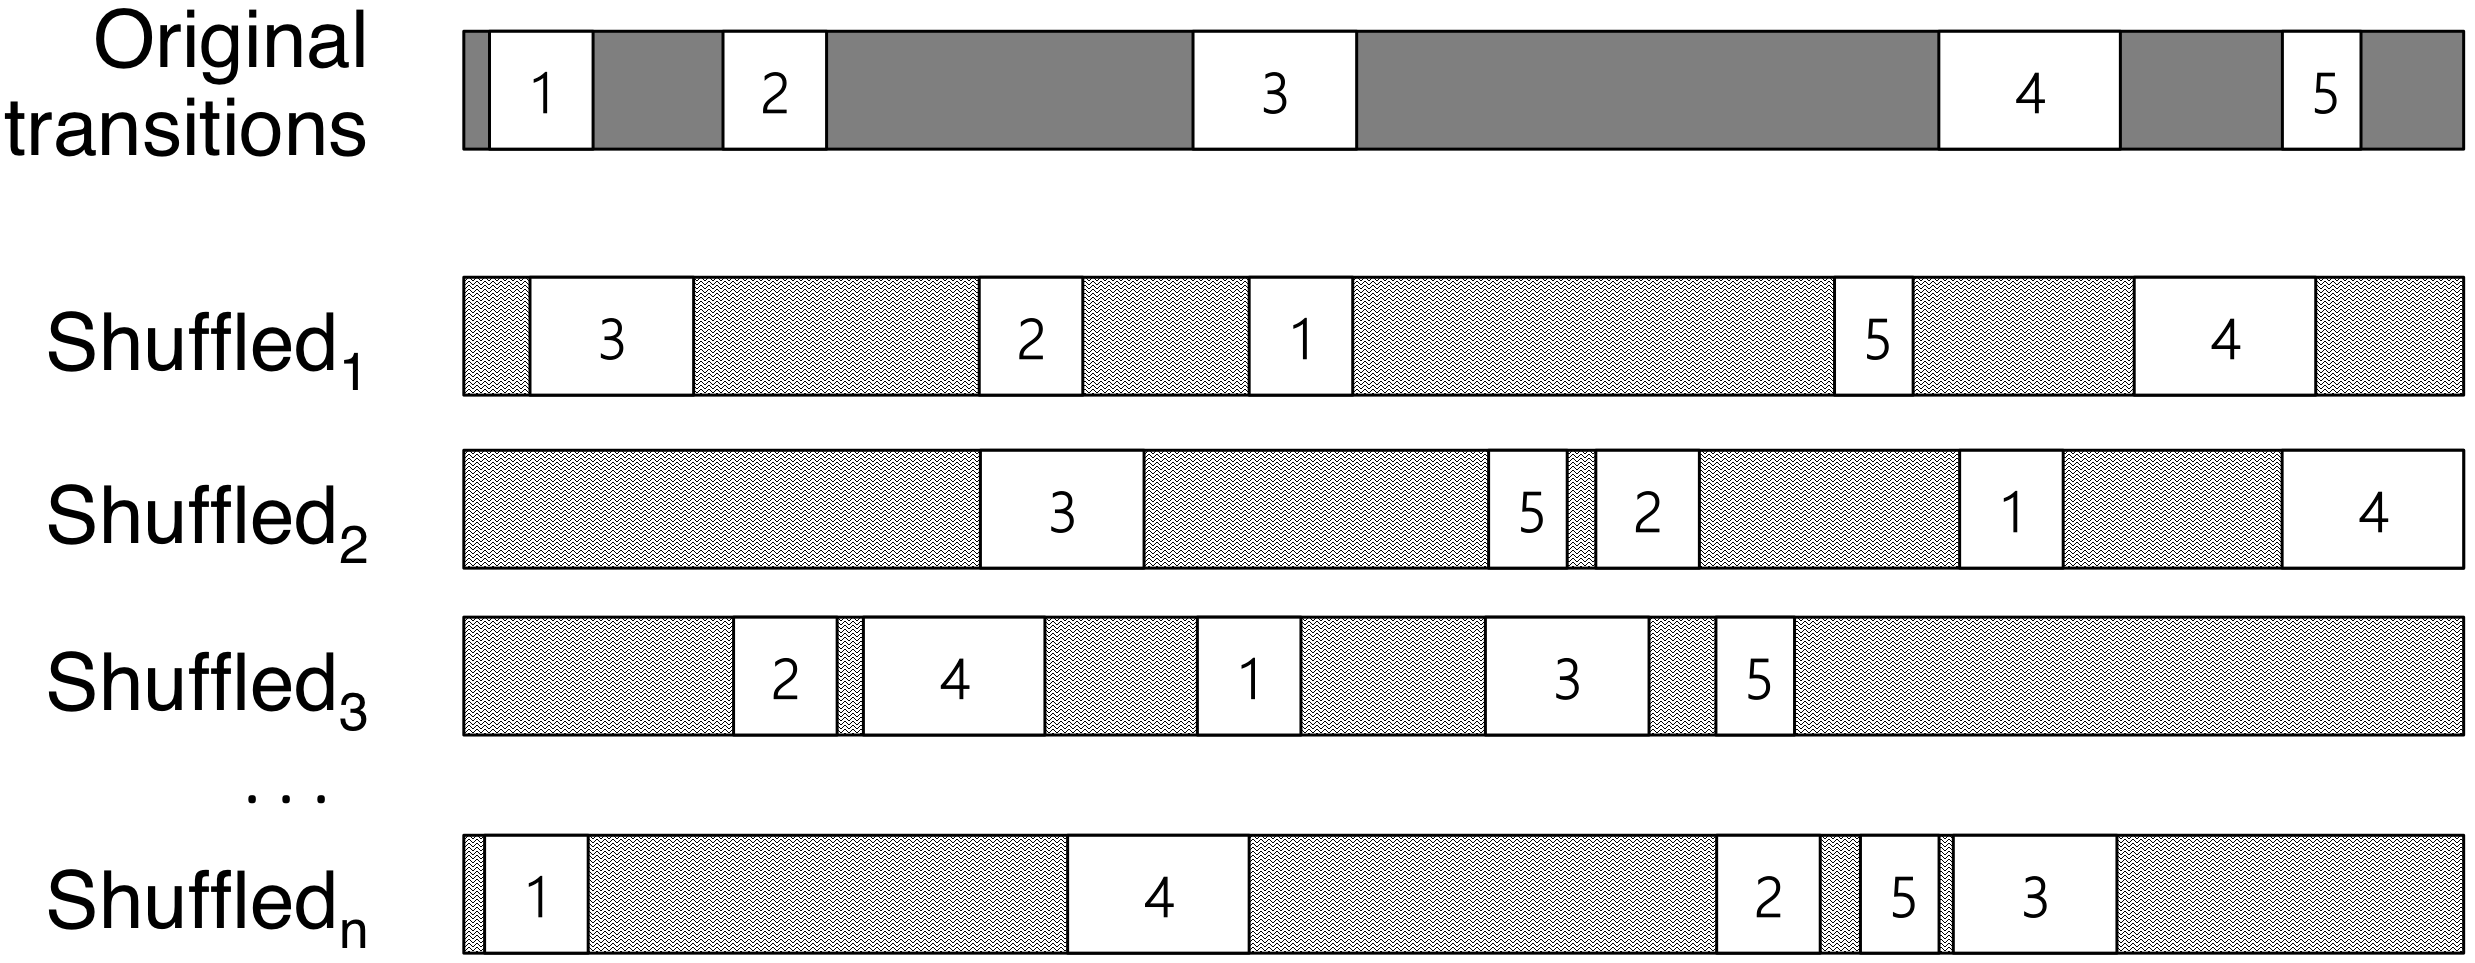
\includegraphics[width=0.8\textwidth]{figures/FIG-ShuffledWindows.png}
\end{center}
\caption{Example of analysis window permutations for a stimulus with five turn transitions. The windows were $\pm$300 msec around the inter-turn gap.} 
\label{fig:shuffling}
\end{figure}

This procedure effectively de-links participants' gaze data from the turn structure in the original stimulus, thereby allowing us to compare turn-related (original) and non-turn-related (randomly permuted) looking behavior using the same eye movement data. The resulting anticipatory gazes from the randomly permuted analysis windows represent an average anticipatory gaze rate over all possible starting points: a random baseline.

By running the real and randomly permuted data sets through identical statistical models, we can estimate how likely it is that predictor effects in the original data (e.g., the effect of language condition; Table \ref{tab:E1-models}) arose from random looking. Because these analyses are complex, we report their full details in \ref{sec:permutation}. 

Our baseline analyses revealed that none of the significant predictors from models of the original, turn-related data can be explained by random looking. For the children's data, the original \textit{z}-values for language condition, gap duration, the age-language condition interaction, and the language condition-transition type interaction were all greater than 95\% of \textit{z}-values for the randomly permuted data (99.9\%, 95.5\%, 99.4\%, and 96\%, respectively, all \textit{p}$<$.05). Similarly, the adults' data showed significant differentiation from the randomly permuted data for two of the three originally significant predictors---transition type and the transition type-gap duration interaction (greater than 99.9\% and 99.7\% of random \textit{z}-values, respectively, all \textit{p}$<$.01)---with marginal differentiation for the interaction of language condition and transition type (greater than 94.6\% of random \textit{z}-values; \textit{p}$=$.054). See Section \ref{sec:permutation} for more information on each predictor's random permutation distribution.

\subsubsection{Developmental effects}

The models reported above revealed a significant interaction of age and language condition (Table \ref{tab:E1-models}) that was unlikely be due to random looking (Figure \ref{fig:E1-randvsreal}). To further explore this effect, we compared the effect of language condition across age groups: using the permuted datasets described above, we extracted the average difference score for the two language conditions (English minus non-English) for each participant, computing an overall average for each random permutation of the data. Then, within each permutation, we made pairwise comparisons of the average difference scores across participant age groups. This process yielded a distribution of random permutation-based difference scores that we could then compare to the difference score in the actual data. Details are given in \ref{sec:pairwisedev}.

These analyses revealed that, while 3- and 4-year olds showed similarly-sized effects of language condition, 5-year-olds had a significantly smaller effect of language condition, compared to both younger age groups. The difference in the language condition effect between 5-year-olds and 3-year-olds was greater than would be expected by chance (99.52\% of the randomly permuted data sets; \textit{p}$<$.01). Similarly, the difference in the language condition effect between 5-year-olds and 4-year-olds was greater than would be expected by chance (99.96\% of the data sets; \textit{p}$<$.001). See Figure \ref{fig:E1-lgageinteraction} for each difference score distribution.

When does spontaneous turn prediction emerge developmentally? To test whether the youngest age group (3-year-olds) already exceeded chance in their anticipatory gaze switches, we compared children's real gaze rates to the random baseline in the English condition with two-tailed \textit{t}-tests. We used the English condition because we are most interested in finding out when children begin to make spontaneous turn predictions for natural speech. We found that three-year-olds made anticipatory gaze switches significantly above chance, when all transitions were considered (\textit{t}(22.824)$=$-4.147, \textit{p}$<$.001) as well as for question transitions alone (\textit{t}(21.677)$=$-5.268, \textit{p}$<$.001).

\subsection{Discussion}
\label{sec:discussion1}

Children and adults spontaneously tracked the turn structure of the conversations, making anticipatory gaze switches at an above-chance rate across all ages and conditions. Children's anticipatory gaze rates were affected by language condition, transition type, age, and gap duration (Table \ref{tab:E1-models}), none of which could be explained by a baseline of random gaze switching (\ref{sec:permutation}; Figure \ref{fig:E1-ChiTs}). These data show a number of important features that bear on our questions of interest. 

First, both adults' and children's anticipations were strongly affected by transition type. Both groups made more anticipatory switches after hearing questions, compared to non-questions. Even in the English videos, when participants had full access to linguistic cues, their rates of anticipation were relatively low (even comparable to the non-English videos) unless the turn was a question. Prior work using online, metalinguistic tasks has shown that participants can use linguistic cues to accurately predict upcoming turn ends \citep{torreira2015, magyari2012, de-ruiter2006}. The current results add a new dimension to our understanding of how listeners make predictions about turn ends: both children and adults spontaneously monitor the linguistic structure of unfolding turns for cues to imminent responses.

Second, children made more anticipatory switches overall in English videos, compared to non-English videos. This effect suggests that lexical access is important for children's ability to anticipate upcoming turn structure, consistent with prior work on turn-end prediction in adults (\citealp{de-ruiter2006}; \citealp{magyari2012}) and children \citep{keitel2013}.

Third, we saw that older children made anticipatory switches more reliably than younger children, but only in the non-English videos. In the English videos, children anticipated well at all ages, especially after hearing questions. This interaction between age and language condition suggests that the 5-year-olds were able to leverage anticipatory cues in the non-English videos in a way that 3- and 4-year-olds could not, possibly by shifting more attention to the non-native prosodic or non-verbal cues. Prior work on children's turn-structure anticipation has proposed that children's turn-end predictions rely primarily on lexicosyntactic structure (and not, e.g., prosody) as they get older \citep{keitel2013}. The current results suggest more flexibility in children's predictions; when they do not have access to lexical information, older children and adults are likely to find alternative cues to turn taking behavior.

In Experiment 2, we follow up on these findings, improving on two aspects of the design: first, our language manipulation in this first experiment was too coarse to provide data regarding specific linguistic channels (e.g., prosody vs. lexicosyntax). In Experiment 2, we compared lexicosyntactic and prosodic cues with phonetically altered speech and used puppets to eliminate non-verbal cues to turn taking. Second, we were not able to pinpoint the emergence of anticipatory switching because the youngest age group in our sample was already able to make anticipatory switches at above chance rates. In Experiment 2, we explore a wider developmental range. 

% Finally, children showed an effect of gap duration (Table \ref{tab:E1-models}). This effect is straightforward: longer gaps resulted in longer analysis windows, yielding more time for children to make an anticipatory gaze.

% Adults' anticipatory gaze rates were also affected by transition type, language condition, and gap duration (Table \ref{tab:E1-models}), none of which could be easily explained by a baseline of random gaze switching (Figure \ref{fig:E1-AduTs}). Like children, adults made more anticipatory switches after hearing questions compared to non-questions, suggesting that anticipation mattered more to them when an immediate response was expected. Also like children, the advantage for questions was driven % by lexical access such that adults must have relied on lexicosyntactic cues to questionhood in picking out turns that potentially require an immediate response, though this effect was only marginally divergent from the distribution of randomly permuted data (\textit{p}$=$.053; Figure \ref{fig:E1-AduTs}). Finally, adults' anticipation rates were also affected by gap duration, but more so for questions than non-questions (Table \ref{tab:E1-models}), suggesting that adults were less likely overall to make switches at non-questions, and so did not benefit from extra time to do so.

% Children and adults' predictions alike were benefited by access to lexical information (English) and speech act status (questionhood), suggesting that linguistic cues, particularly lexical ones, facilitate their spontaneous predictions about upcoming turn structure through the identification of turns with immediate responses. Children's anticipatory gaze rates for questions and non-questions in English was stable across ages and comparable to adult behavior (Figure \ref{fig:E1-randvsreal}), suggesting that they can identify questions in native stimuli with adult-like competence by age three. Although participants' ability to recognize questions was facilitated by lexical access (i.e., English vs. non-English), the prosody in the non-English videos was non-native, and so the experimental design can not conclusively show which linguistic cues children relied on in the English videos to identify question turns. Relatedly, though lexical access clearly facilitated participants' anticipatory gaze rate, it was not necessary for participants---especially adults---in order to exceed chance switching rates (Figure \ref{fig:E1-randvsreal}), suggesting that participants use non-lexical cues (e.g., prosody, non-verbal behavior) to make anticipatory eye movements at least some of the time.

\section{Experiment 2}
\label{sec:exp2}

Experiment 2 used native-language stimuli, controlled for lexical and prosodic information, eliminating non-verbal cues, and tested children from a wider age range. To tease apart the role of lexical and prosodic information, we phonetically manipulated the speech signal for pitch, syllable duration, and lexical access. By testing 1- to 6-year-olds we hoped to find the developmental onset of turn-predictive gaze. We also hoped to measure changes in the relative roles of prosody and lexicosyntax across development.

Non-verbal cues in Experiment 1 (e.g., gaze and gesture) could have helped participants make predictions about upcoming turn structure  \citep{rossano2009, stivers2010}. Since our focus was on linguistic cues, we eliminated all gaze and gestural signals in Experiment 2 by replacing the videos of human actors with videos of puppets. Puppets are less realistic and expressive than human actors, but they create a natural context for having somewhat motionless talkers in the videos (thereby allowing us to eliminate gestural and gaze cues). Additionally, the prosody-controlled condition included small but global changes to syllable duration that would have required complex video manipulation or precise re-enactment with human talkers, neither of which was feasible. For these reasons, we decided to substitute puppet videos for human videos in the final stimuli. 

As in the first experiment, we recorded participants' eye movements as they watched six short videos of dyadic conversation, and then analyzed their anticipatory glances from the current speaker to the upcoming speaker at points of turn transition.

\subsection{Methods}
\label{sec:methods2}

\subsubsection{Participants}
We recruited 27 undergraduate adults and 129 children between ages 1;0--6;11 to participate in our experiment. We recruited our child participants from the Children's Discovery Museum of San Jose, California\footnote{We ran Experiment 2 at a local children's museum because it gave us access to children with a more diverse range of ages.}, targeting approximately 20 children for each of the six one-year age groups (range: 20--23). All participants were native English speakers, though some parents (N$=$27) reported that their child heard a second (and sometimes third) language at home. None of the adult participants reported fluency in a second language.

\begin{figure}[t]
\begin{center}
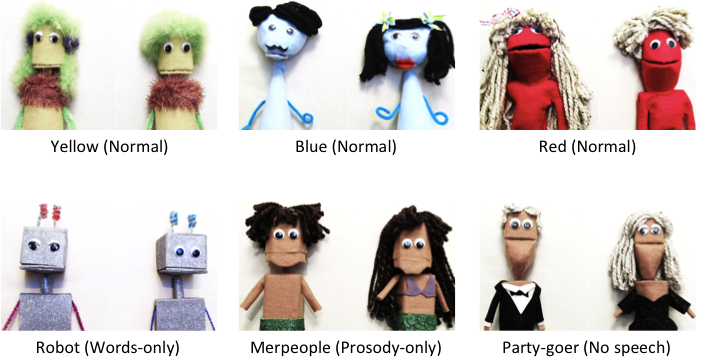
\includegraphics[width=\textwidth]{figures/FIG-EN-stim.png}
\end{center}
\caption{The six puppet pairs (and associated audio conditions). Each pair was linked to three distinct conversations from the same condition across the three experiment versions.}
\label{fig:puppets}
\end{figure}

\subsubsection{Materials}
We created 18 short videos of improvised, child-friendly conversation (Figure \ref{fig:puppets}). To eliminate non-verbal cues to turn transition and to control the types of linguistic information available in the stimuli we first audio-recorded improvised conversations, then phonetically manipulated those recordings to limit the availability of prosodic and lexical information, and finally recorded video to accompany the manipulated audio, featuring puppets as talkers. 

\textit{Audio recordings}. The recording session was set up in the same way as the first experiment, but with a shorter warm up period (5--10 minutes) and a pre-determined topic for the child-friendly improvisation (`riding bikes', `pets', `breakfast', `birthday cake', `rainy days', or `the library'). All of the talkers were native English speakers, and were recorded in male-female pairs. As before, we asked talkers to speak ``as if they were on a children's television show'' and to ask at least a few questions during the improvisation. We cut each audio recording down to the (approximate) 20-second interval with the most turn activity. The 20-second clips were then phonetically manipulated and used in the final video stimuli.

\textit{Audio Manipulation}. We created four versions of each audio clip: \textit{normal}, \textit{words only}, \textit{prosody only}, and \textit{no speech}. That is, one version with a full linguistic signal (\textit{normal}), and three with incomplete linguistic information (hereafter ``partial cue'' conditions). The \textit{normal} clips were the unmanipulated, original audio clips. 

The \textit{words only} clips were manipulated to have robot-like speech: we flattened the intonation contours to each talker's average pitch (F$_{0}$) and we reset the duration of every nucleus and coda to each talker's average nucleus and coda duration.\footnote{We excluded hyper-lengthened words like [w\textipa{aU:}] `woooow!'. These were rare in the clips.} We made duration and pitch manipulations using PSOLA resynthesis in Praat \citep{Praat}. Thus, the \textit{words only} versions of the audio clips had no pitch or durational cues to upcoming turn boundaries, but did have intact lexicosyntactic cues (and residual phonetic correlates of prosody, e.g., intensity). 

We created the \textit{prosody only} clips by low-pass filtering the original recording at 500 Hz with a 50 Hz Hanning window (following de Ruiter et al., 2006). This manipulation creates a ``muffled speech'' effect because low-pass filtering removes most of the phonetic information used to distinguish between phonemes. The \textit{prosody only} versions of the audio clips lacked lexical information, but retained their intonational and rhythmic cues to upcoming turn boundaries. 

The \textit{no speech} condition served as a non-linguistic baseline. For this condition, we replaced the original clip with multi-talker babble: we overlaid multiple child-oriented conversations (not including the original one), and then cropped the result to the duration of the original video. Thus, the \textit{no speech} audio clips lacked any linguistic information to upcoming turn boundaries---the only cue to turn taking was the opening and closing of the puppets' mouths. 

Finally, because low-pass filtering removes significant acoustic energy, the \textit{prosody only} clips were much quieter than the other three conditions. Our last step was to downscale the intensity of the audio tracks in the three other conditions to match the volume of the \textit{prosody only} clips. We referred to the conditions as ``normal'', ``robot'', ``mermaid'', and ``birthday party'' speech when interacting with participants.

\textit{Video recordings}. We created puppet video recordings to match the manipulated 20-second audio clips. The puppets were minimally expressive; so that the puppeteer could only control the opening and closing of their mouths; the puppets' heads, eyes, arms, and bodies stayed still. Puppets were positioned looking forward to eliminate shared gaze as a cue to turn structure \citep{thorgrimsson2015}. We took care to match the puppets' mouth movements to the syllable onsets as closely as possible, specifically avoiding any mouth movement before the onset of a turn. We then added the manipulated audio clips to the puppet video recordings by hand.

We used three pairs of puppets used for the \textit{normal} condition---`red', `blue' and `yellow'---and one pair of puppets for each partial cue condition: ``robots'', ``merpeople'', and ``party-goers'' (Figure 8). We randomly assigned half of the conversation topics (`birthday cake', `pets', and `breakfast') to the \textit{normal} condition, and half to the partial cue conditions (`riding bikes', `rainy days', and `the library'). We then created three versions of the experiment, so that each of the six puppet pairs was associated with three different conversation topics across the different versions of the experiment (18 videos in total). We ensured that the position of the talkers (left and right) was counterbalanced in each version by flipping the video and audio channels as needed.

The duration of turn transitions and the number of speaker changes across videos was variable because the conversations were recorded semi-spontaneously. We measured turn transitions from the audio signal of the \textit{normal}, \textit{words only}, and \textit{prosody only} conditions. There was no audio from the original conversation in the \textit{no speech} condition videos, so we measured turn transitions from puppets' mouth movements in the video signal, using ELAN video annotation software \citep{ELAN}.

There were 85 turn transitions for analysis after excluding transitions longer than 550 msec and shorter than 90 msec. The remaining turn transitions had more questions than non-questions (N$=$47 and N$=$38, respectively), with transitions distributed somewhat evenly across conditions (keeping in mind that there were three \textit{normal} videos and only one partial cue video for each experiment version): \textit{normal} (N$=$36), \textit{words only} (N$=$13), \textit{prosody only} (N$=$17), and \textit{no speech} (N$=$19). Inter-turn gaps for questions (mean$=$366, median$=$438, stdev$=$138 msec) were longer than those for non-questions (mean$=$305, median$=$325, stdev$=$94 msec) on average, but gap duration was overall comparable across conditions: \textit{normal} (mean$=$334, median$=$321, stdev$=$130 msec), \textit{words only} (mean$=$347, median$=$369, stdev$=$ 115 msec), \textit{prosody only} (mean$=$365, median$=$369, stdev$=$104 msec), and \textit{no words} (mean$=$319, median$=$329, stdev$=$136 msec). The longer gaps for question transitions could give them an advantage because our anticipatory measure includes shifts initiated during the gap between turns (Figure \ref{fig:criterion}).

\subsection{Procedure}
We used the same experimental apparatus and procedure as in the first experiment. Each participant watched six puppet videos in random order, with five 15--30 second filler videos placed in-between (e.g., running puppies, moving balls, flying bugs). Three of the puppet videos had \textit{normal} audio while the other three had \textit{words only}, \textit{prosody only}, and \textit{no speech} audio. This experiment required no special instructions so, as before, the experimenter immediately began each session with calibration and then stimulus presentation. The entire experiment took less than five minutes.

\linespread{1}
\begin{table}[t]
\begin{center}
  \begin{tabular}{llcccc}
    \hline
    Age group & Speaker & Addressee & Other onscreen & Offscreen\\ 
    \hline
    1 & 0.44 & 0.14 & 0.23 & 0.19 \\ 
    2 & 0.50 & 0.13 & 0.24 & 0.14 \\ 
    3 & 0.47 & 0.12 & 0.25 & 0.16 \\ 
    4 & 0.48 & 0.11 & 0.29 & 0.12 \\ 
    5 & 0.54 & 0.11 & 0.20 & 0.14 \\ 
    6 & 0.60 & 0.12 & 0.18 & 0.10 \\
    Adult & 0.69 & 0.12 & 0.09 & 0.10 \\
%   Overall & 0.53 & 0.12 & 0.21 & 0.13 \\
    \hline
  \end{tabular}
\end{center}
  \caption{Average proportion of gaze to the current speaker and addressee during periods of talk across ages.}
\label{tab:look_e2}
\end{table}
\linespread{2}

\linespread{1}
\begin{table}
\begin{center}
  \begin{tabular}{llcccc}
    \hline
    Condition & Speaker & Addressee & Other onscreen & Offscreen\\ 
    \hline
    Normal 				& 0.58 & 0.12 & 0.17 & 0.13 \\ 
    Words only 		& 0.54 & 0.11 & 0.24 & 0.10 \\ 
    Prosody only 	& 0.48 & 0.12 & 0.26 & 0.15 \\ 
    No speech 		& 0.44 & 0.13 & 0.26 & 0.18 \\
    \hline
  \end{tabular}
\end{center}
  \caption{Average proportion of gaze to the current speaker and addressee during periods of talk across conditions.}
\label{tab:look_e2b}
\end{table}
\linespread{2}

% Average prop gaze to the current speaker across conditions for one-year-olds
%                           speaker addressee other-screen offscreen
%Normal   		  0.4737582 0.1366432    0.2003952 0.1892035
%Words only    0.3977261 0.1283417    0.3112005 0.1627317
%Prosody only 0.4290202 0.1611453    0.2558657 0.1539688
%No speech    0.3786925 0.1228615    0.2356423 0.2628037

\subsubsection{Data preparation and coding}
We coded each turn transition for its linguistic condition (\textit{normal}, \textit{words only}, \textit{prosody only}, and \textit{no speech}) and transition type (question/non-question)\footnote{We coded \textit{wh-}questions as ``non-questions'' for the \textit{prosody only} videos. Polar questions often have a final rising intonational contour, but \textit{wh-}questions often do not  \citep{hedberg2010}.}, and identified anticipatory gaze switches to the upcoming speaker using the methods from Experiment 1.

\begin{figure}[!ht]
\begin{center}
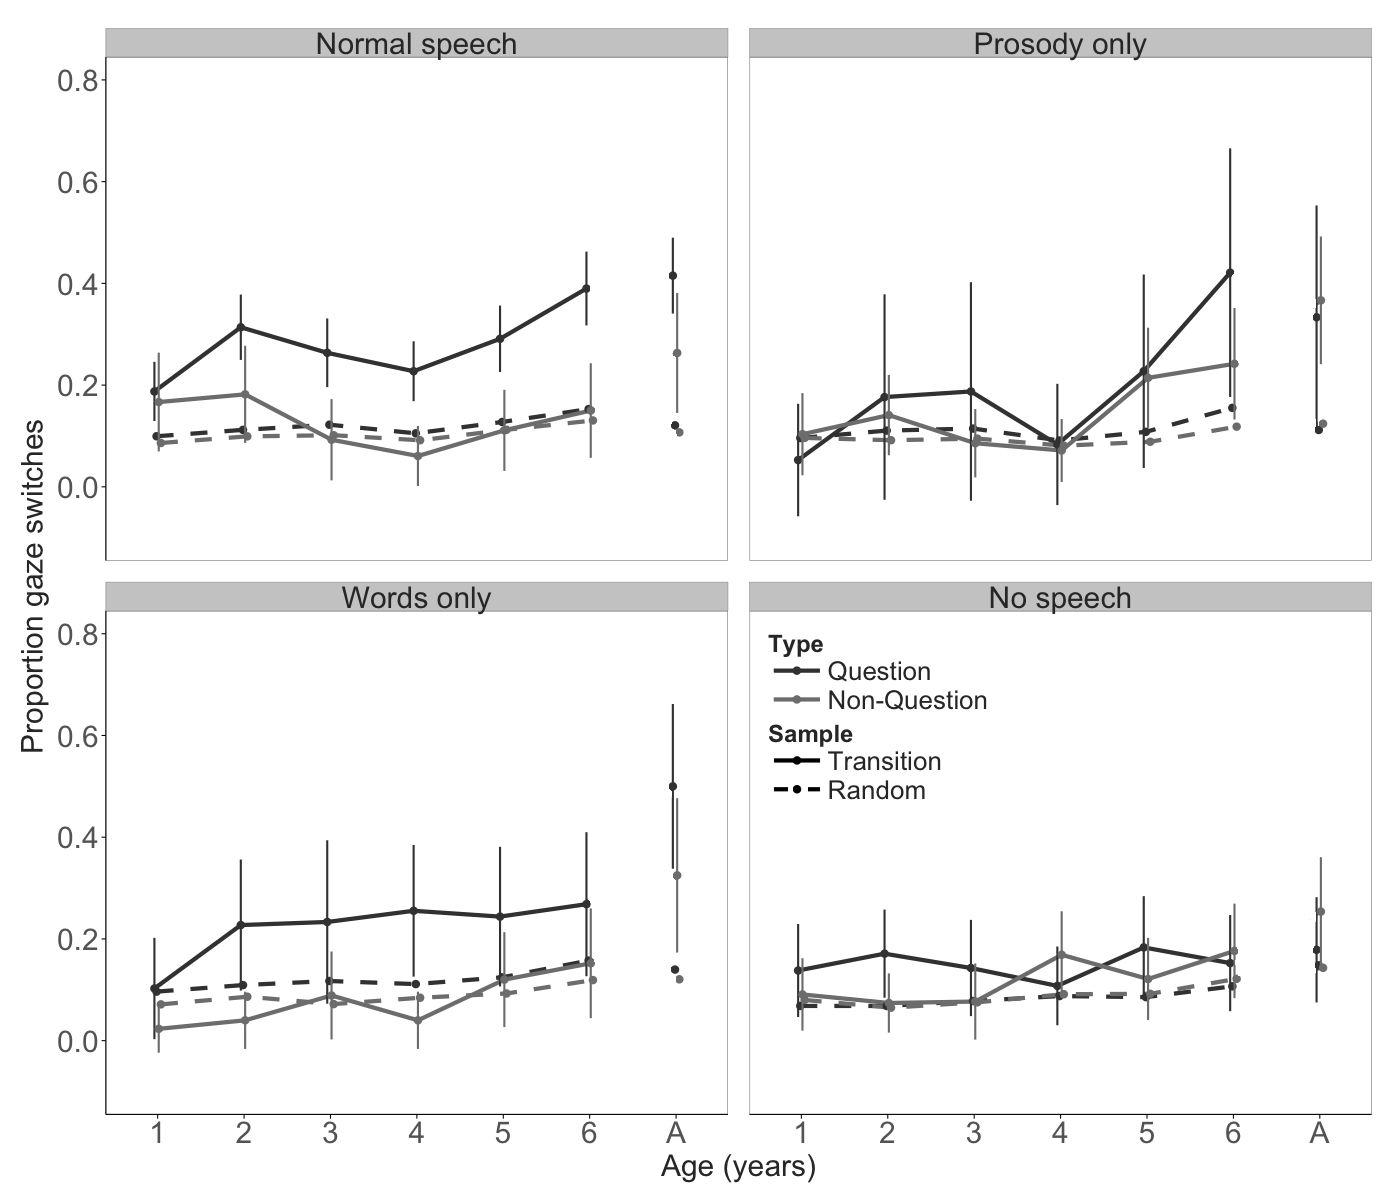
\includegraphics[width=\textwidth]{figures/E2-samples-by-lang-groups-trans-types.png}
\end{center}
\caption{Anticipatory gaze rates across language condition and transition type for the real data (blue, dark green, light green, and red) and the randomly permuted baselines (gray). Vertical bars represent 95\% confidence intervals.} 
\label{fig:E2-randvsreal}
\end{figure}

\subsection{Results}
\label{sec:results2}

Participants' pattern of gaze indicated that they performed basic turn tracking across all ages and in all conditions. Participants looked at the screen most of the time during video playback (82\% and 86\% average for children and adults, respectively), primarily looking at the person who was currently speaking (Table 2). They tracked the current speaker in every condition---even one-year-olds looked more at the current speaker than at anything else in the three partial cue conditions (40\% for \textit{words only}, 43\% for \textit{prosody only}, and 39\% for \textit{no speech}). There was a steady overall increase in looks to the current speaker with age and added linguistic information (Tables \ref{tab:look_e2} and \ref{tab:look_e2b}). Looks to the addressee also decreased with age, but the change was minimal. Figure \ref{fig:E2-randvsreal} shows participants' anticipatory gaze rates across age, the four language conditions, and transition type.

\subsubsection{Statistical models}
\label{sec:models2}

We identified anticipatory gaze switches for all 85 usable turn transitions, and analyzed them for effects of language condition, transition type, and age with two mixed-effects logistic regressions. We again built separate models for children and adults because effects of age were only pertinent to the children's data. The child model included condition (\textit{normal}/\textit{prosody only}/\textit{words only}/\textit{no speech}; with \textit{no speech} as the reference level), transition type (question vs. non-question), age (1, 2, 3, 4, 5, 6; numeric), and duration of the inter-turn gap (in seconds) as predictors, with full interactions between language condition, transition type, and age.  We again included the duration of the inter-turn gap as a control predictor and added random effects of item (turn transition) and participant, with random slopes of transition type for participants. The adult model included condition, transition type, their interactions, and duration as a control predictor, with participant and item included as random effects and random slopes of condition and transition type.

Children's anticipatory gaze switches showed an effect of gap duration (\textit{$\beta$}=3.95, \textit{SE}=0.617, \textit{z}=6.401, \textit{p}$<$.001), a two-way interaction of age and language condition (for \textit{prosody only} speech compared to the \textit{no speech} reference level; \textit{$\beta$}=0.393, \textit{SE}=0.189, \textit{z}=2.08, \textit{p}$<$.05), and a three-way interaction of age, transition type, and language condition (for \textit{normal} speech compared to the \textit{no speech} reference level; \textit{$\beta$}=-0.38, \textit{SE}=0.17, \textit{z}=-2.229, \textit{p}$<$.05). There were no significant effects of age or transition type alone (Table \ref{sec:models2}), with only a marginal effect of language condition (for \textit{prosody only} compared to the \textit{no speech} reference level; \textit{$\beta$}=-1.607, \textit{SE}=0.867, \textit{z}=-1.85, \textit{p}$=$.064)

Adults' anticipatory gaze switches showed effects of gap duration (\textit{$\beta$}=4.7, \textit{SE}=1.18, \textit{z}=3.978, \textit{p}$<$.001) and language condition (for \textit{normal} speech \textit{$\beta$}=1.203, \textit{SE}=0.536, \textit{z}=2.245, \textit{p}$<$.05 and \textit{words only} speech \textit{$\beta$}=1.561, \textit{SE}=0.709, \textit{z}=2.203, \textit{p}$<$.05  compared to the \textit{no speech} reference level). There were no effects of transition type (\textit{$\beta$}=0.437, \textit{SE}=0.585, \textit{z}=0.747, \textit{p}$=$.45).

\subsubsection{Random baseline comparison}
\label{sec:randbaseline2}

Using the same technique described in Experiment 1 (Section \ref{sec:randbaseline1}), we created and modeled random permutations of participants' anticipatory gaze. These analyses revealed that none of the significant predictors from models of the original, turn-related data could be explained by random looking. In the children's data, the original model's \textit{z}-values for language condition (\textit{prosody only}), gap duration, the two-way interaction of age and language condition (\textit{prosody only}) and the three-way interaction of age, transition type, and language condition (\textit{normal} speech) were all greater than 95\% of the randomly permuted \textit{z}-values (96.5\%, 100\%, 95.6\%, and 95.5\%, respectively, all \textit{p}$<$.05). Similarly, the adults' data showed significant differentiation from the randomly permuted data for all originally significant predictors: gap duration and language condition for \textit{normal} speech and \textit{words only} speech (greater than 100\%, 97.8\%, and 99.1\% of random \textit{z}-values, respectively, all \textit{p}$<$.05). See Section \ref{sec:permutation} for more information on each predictor's random permutation distribution.

\linespread{1}
\begin{minipage}[t]{0.95\linewidth}
\begin{footnotesize}
\begin{longtable}{lcccl}
  \textbf{\textit{Children}} &&&& \\
    \hline
           &  Estimate & Std. Error & \textit{z} value & Pr($>$$|$\textit{z}$|$) \\    
    \hline
    (Intercept)											& -3.49403		& 0.48454		& -7.211	& 5.55e-13 ***    	\\
    Age														& 0.02436		& 0.10249		& 0.238	& 0.8121        		\\
    Type$=$\textit{non-Question}			& -0.88900		& 0.61192		& -1.453	& 0.1463        		\\
    GapDuration												& 3.94743		& 0.61668		& 6.401	& 1.54e-10 ***    	\\
    Age*Type$=$\textit{non-Question}	& 0.15359		& 0.13996		& 1.097	& 0.2725        		\\
	\hline
    Condition$=$\textit{normal}				& 0.37337		& 0.43421		& 0.860	& 0.3899        		\\
    Age*Condition$=$\textit{normal}		& 0.12950		& 0.10217		& 1.267	& 0.2050        		\\
    Condition$=$\textit{normal}*			& 0.91074		& 0.72581		& 1.255	& 0.2096        		\\
    \hspace*{5mm} Type$=$\textit{non-Question} &&&& \\
    Age*Condition$=$\textit{normal}*	& -0.37965		& 0.17031		& -2.229	& 0.0258 *      		\\
    \hspace*{5mm} Type$=$\textit{non-Question} &&&& \\
	\hline
    Condition$=$\textit{prosody}			& -1.60734		& 0.86680		& -1.854	& 0.0637 .      		\\
    Age*Condition$=$\textit{prosody}	& 0.39271		& 0.18905		& 2.077	& 0.0378 *      		\\
    Condition$=$\textit{prosody}*			& 1.68552		& 1.05414		& 1.599	& 0.1098        		\\
    \hspace*{5mm} Type$=$\textit{non-Question} &&&& \\
    Age*Condition$=$\textit{prosody}*	& -0.32360		& 0.23229		& -1.393	& 0.1636        		\\
    \hspace*{5mm} Type$=$\textit{non-Question} &&&& \\
	\hline
    Condition$=$\textit{words}				& -0.26996		& 0.59313		& -0.455	& 0.6490        		\\
    Age*Condition$=$\textit{words}		& 0.14044		& 0.13565		& 1.035	& 0.3005        		\\
    Condition$=$\textit{words}*				& -1.03066		& 1.01610		& -1.014	& 0.3104        		\\
    \hspace*{5mm} Type$=$\textit{non-Question} &&&& \\
    Age*Condition$=$\textit{words}*		& 0.08829		& 0.22387		& 0.394	& 0.6933        		\\
    \hspace*{5mm} Type$=$\textit{non-Question} &&&& \\
    \hline
  &&&& \\
  \textbf{\textit{Adults}} &&&& \\
    \hline
           &  Estimate & Std. Error & \textit{z} value & Pr($>$$|$\textit{z}$|$) \\    
    \hline
    (Intercept)											& -3.3811		& 0.6884		& -4.912	& 9.03e-07 *** 		\\ 
    Type$=$\textit{non-Question}			& 0.4375			& 0.5854		& 0.747	& 0.4549     		\\ 
    GapDuration												& 4.6961			& 1.1804		& 3.978	& 6.94e-05 *** 		\\ 
	\hline
    Condition$=$\textit{normal}				& 1.2033			& 0.5359		& 2.245	& 0.0247 *   		\\ 
    Condition$=$\textit{normal}*			& -0.9627		& 0.7358		& -1.308	& 0.1907     		\\ 
    \hspace*{5mm} Type$=$\textit{non-Question} &&&& \\
	\hline
    Condition$=$\textit{prosody}			& 0.2407			& 0.8011		& 0.301	& 0.7638     		\\ 
    Condition$=$\textit{prosody}*			& 0.5525			& 0.9374		& 0.589	& 0.5556     		\\ 
    \hspace*{5mm} Type$=$\textit{non-Question} &&&& \\
	\hline
    Condition$=$\textit{words}				& 1.5613			& 0.7087		& 2.203	& 0.0276 *   		\\ 
    Condition$=$\textit{words}*				& -1.1557		& 0.8854		& -1.305	& 0.1918     		\\ 
    \hspace*{5mm} Type$=$\textit{non-Question} &&&& \\
    \hline
    &&&& \\
  \caption{Model output for children and adults' anticipatory gaze switches in Experiment 2.}
\label{tab:E2-models}
\end{longtable}
\end{footnotesize}
\end{minipage}
\linespread{2}

\subsubsection{Developmental effects}

Our main goal in extending the age range to 1- and 2-year-olds in Experiment 2 was to find the age of emergence for spontaneous predictions about upcoming turn structure. As in Experiment 1, we used two-tailed \textit{t}-tests to compare children's real gaze rates to the random baseline rates in the \textit{normal} speech condition, in which the speech stimulus is most like what children hear every day. We tested real gaze rates against baseline for three age groups: ages one, two, and three. Two- and three-year-old children made anticipatory gaze switches significantly above chance both when all transitions were considered (2-year-olds: \textit{t}(26.193)$=$-4.137, \textit{p}$<$.001; 3-year-olds: \textit{t}(22.757)$=$-2.662, \textit{p}$<$.05) and for question transitions alone (2-year-olds: \textit{t}(25.345)$=$-4.269, \textit{p}$<$.001; 3-year-olds: \textit{t}(21.555)$=$-3.03, \textit{p}$<$.01). One-year-olds, however, only made anticipatory gaze shifts marginally above chance for turn transitions overall and for question turns alone (overall: \textit{t}(24.784)$=$-2.049, \textit{p}$=$.051; questions: \textit{t}(25.009)$=$-2.03, \textit{p}$=$.053).

The regression models for the children's data also revealed two significant interactions with age. The first was a significant interaction of age and language condition (for \textit{prosody only} compared to the \textit{no speech} reference level), suggesting a different age effect between the two linguistic conditions. As in Experiment 1, we explored each age interaction by extracting an average difference score over participants for the effect of language condition (\textit{no speech} vs. \textit{prosody only}) within each random permutation of the data, making pairwise comparisons between the six age groups. These tests revealed that children's anticipation in the \textit{prosody only} condition significantly improved at ages five and six (with difference scores greater than 95\% of the random data scores; \textit{p}$<$.05). See Figure \ref{fig:E2-lgageinteraction} for these \textit{prosody only} difference score distributions.

The second age-based interaction was a three-way interaction of age, transition type, and language condition (for \textit{normal} speech compared to the \textit{no speech} baseline). We again created pairwise comparisons of the average difference scores for the transition type-language condition interaction across age groups in each random permutation of the data, finding that the effect of transition type in the \textit{normal} speech condition became larger with age, with significant improvements by age 4 over ages 1 and 2 (99.9\% and 98.86\%, respectively), by age 5 over age 4 (97.54\%), and by age 6 over ages 1, 2, and 5 (99.5\%, 97.36\%, and 95.04\%), all significantly different from chance (\textit{p}$<$.05). See Figure \ref{fig:E2-lgagetypeinteraction} for these \textit{normal} speech difference score distributions.

\subsection{Discussion}
\label{sec:discussion2}

The core aims of Experiment 2 were to gain better traction on the individual roles of prosody and lexicosyntax in children's turn predictions, and to find the age of emergence for spontaneous turn anticipation. Many of our results replicate the findings from Experiment 1: participants often made more anticipatory switches when they had access to lexical information and, when they did, tended to make more anticipatory switches for questions compared to non-questions. 

As in Experiment 1, children and adults spontaneously tracked the turn structure of the conversations, making anticipatory gaze switches at above-chance rates across all ages when listening to natural speech. They also made far more anticipations for questions than for non-question turns---at least for children two years old and older. But these effects were different for the two conditions with partial linguistic information: \textit{prosody only} and \textit{words only}. In the \textit{prosody only} condition, performance was low for younger children and increased significantly with age (especially for questions). In the \textit{words only} condition, children age two and older showed robust anticipatory switching for questions (much like in \textit{normal} speech), but never rose above chance for non-question turns. These findings do not therefore support an early role for prosody in children's spontaneous turn structure predictions. There is also no evidence that lexical information is sufficient on its own to support children's anticipatory switching.

\section{General Discussion}
\label{sec:gendisc}

Children begin to develop conversational turn-taking skills long before their first words emerge \citep{bateson1975, hilbrink2015, jaffe2001, snow1977}. As they acquire language, they also acquire the information needed to make accurate predictions about upcoming turn structure. Until recently, we have had very little data on how children weave language into their already-existing turn-taking behaviors. In two experiments investigating children's anticipatory gaze to upcoming speakers, we found evidence that turn prediction develops early in childhood and that spontaneous predictions are primarily driven by participants' expectation of an immediate response in the next turn (e.g., after questions). In making predictions about upcoming turn structure, children used a combination of lexical and prosodic cues; neither lexical nor prosodic cues alone were sufficient to support increased anticipatory gaze. We also found no early advantage for prosody over lexicosyntax, and instead found that children were unable to make above-chance anticipatory gazes in the \textit{prosody only} condition until age five. We discuss these findings with respect to the role of linguistic cues in predictions about upcoming turn structure, the importance of questions in spontaneous predictions about conversation, and children's developing competence as conversationalists.

\subsection{Predicting turn structure with linguistic cues}

Prior work with adults has found a consistent role for lexicosyntax in predicting upcoming turn structure \citep{de-ruiter2006, magyari2012}, whereas the role of prosody still under debate \citep{duncan1972, ford1996, torreira2015}. Knowing that children comprehend more about prosody than lexicosyntax early on (Section \ref{sec:intro}; also see \citealp{speer2009} for a review), we thought it possible that young children would instead show an advantage for prosody in their predictions about turn structure in conversation. Our results suggest that, on the contrary, exclusively presenting prosodic information to children limits their spontaneous predictions about upcoming turn structure until age five.

Perhaps surprisingly, we also found no evidence that lexical information alone is equivalent to the full linguistic signal in driving children's predictions, as has been shown previously for adults \citep{magyari2012, de-ruiter2006} and as is replicated with adult participants in the current study. That said, our findings point more toward early lexical effects in children's turn anticipations than prosodic ones: children's performance in both experiments was consistently better when they had access to lexical information, especially after question turns. And although the \textit{words only} condition in Experiment 2 was not significantly different from the baseline \textit{no speech} condition, children's anticipations trended toward above-chance rates.

Above all, children and adults anticipated best with they had access to the full linguistic signal. There may be something informative about combined prosodic and lexical cues to questionhood that helps to boost children's anticipations before they can use these cues separately. Even in adults, Torreira and colleagues (\citeyear{torreira2015}) showed that the trade-off in informativity between lexical and prosodic cues is more subtle in semi-natural speech. The present findings are the first to show evidence of a similar effect developmentally.

\subsection{The question effect}

In both experiments, anticipatory looking was primarily driven by question transitions, a pattern that has not been previously reported in other anticipatory gaze studies, on children or adults (Keitel et al., 2013; Hirvenkari, 2013; Tice and Henetz, \citeyear{TiceHenetz11}). Questions make an upcoming speaker switch immediately relevant, helping the listener to predict with high certainty what will happen next (i.e., an answer from the addressee), and are often easily identifiable by overt prosodic and lexicosyntactic cues.

Compared to prosodic cues (e.g., final rising intonation), lexicosyntactic cues to questionhood (e.g., \textit{wh}-words, \textit{do}-insertion, and subject-auxiliary inversion) are categorical, and early-occurring in the utterance. Children may have therefore had an easier time picking out and interpreting lexical cues to questionhood. Developmentally, the question effect showed its first significant gains between ages three and four in the \textit{normal} speech condition of Experiment 2 (Figure \ref{fig:E2-lgagetypeinteraction}), by which time children frequently hear and use a variety of polar and \textit{wh}-questions \citep{clark2009}. Furthermore, while lexicosyntactic question cues were available on every instance of \textit{wh}- and \textit{yes/no} questions in our stimuli, prosodic question cues were only salient on \textit{yes/no} questions. Finally, the mapping of prosodic contour to speech act (e.g., high final rises for polar questions) is far from one-to-one, leaving substantial room for uncertainty in prosodic contour interpretation in general.

Prior work on children's acquisition of questions indicates that they may already have some knowledge of question-answer sequences by the time they begin to speak: questions make up approximately one third of the utterances children hear, before and after the onset of speech, and even into their preschool years, though the type and complexity of questions changes throughout development \citep{casillas2016, fitneva2012, henning2005, shatz1979}.\footnote{There is substantial variation in question frequency by individual and socioeconomic class \citep{hart1992, weisleder2012}.} For the first few years, many of the questions directed to children are ``test'' questions---questions that the caregiver already has the answer to (e.g., ``What does a cat say?''), but this changes as children get older. Questions help caregivers to get their young children's attention and to ensure that information is in common ground, even if the responses are non-verbal or infelicitous \citep{bruner1985, fitneva2012, snow1977}. So, in addition to having a special interactive status (for adults and children alike), questions are a core characteristic of many caregiver-child interactions, motivating a general benefit for questions in turn structure anticipation.

Two important questions for future work are then: (1) how does children's ability to monitor for questions in conversation relate to their prior experience with questions? and (2) what is it about questions that makes children and adults more likely to anticipatorily switch their gaze to addressees? Other turn types, such as imperatives, compliments, and complaints make a response from the addressee highly likely in the next turn \citep{schegloff2007}. Rhetorical and tag questions, on the other hand, take a similar form to prototypical polar questions, but often do not require an answer. So, though it is clear that adults and children anticipated responses more often for questions than non-questions, we do not yet know whether their predictive action is limited to turns formatted as questions or is generally applicable to turn structures that project an immediate response from the addressee. 

More broadly, our results suggest that participants' spontaneous predictions, at least while viewing third-party conversation, are driven by what lies \textit{beyond} the end of the current turn---not just by the upcoming end of the turn itself, as has been focused on in prior work \citep{torreira2015, keitel2013, magyari2012, de-ruiter2006}. In future work, it will be crucial to measure prediction from a first-person perspective to resolve this apparent contradiction (see also \citealp{holler2015}).

% There is at least one clear hypothesis that can bridge these apparently conflicting results: listeners in spontaneous, first-person conversation may use multiple strategies in making predictions about upcoming turn structure, using more passive prediction to detect upcoming speaker transition (e.g., questions), and then switching into precise turn-end prediction mode (\`{a} la \citealp{de-ruiter2006}) when necessary. A flexible prediction system like this one allows listeners to continuously monitor ongoing conversation at a low cost while still managing to plan their responses and come in quickly when needed.

% To test this hypothesis, which integrates findings from turn-structure prediction with multiple measures, age groups, and styles of linguistic control, it will be crucial to look at prediction from a first-person perspective. The results we present here are based on predictions about third-party conversation, which enables participants to follow interactions with no chance of actually participating. Although recent work has shown that similar anticipatory eye gazes do occur in spontaneous conversation \citep{holler2015}, more work is needed to determine if the same question advantage occurs, which linguistic cues seem to drive it, and whether participants switch into a ``precision'' mode when they detect imminent speaker change.

\subsection{Early competence for turn taking?}

One of the core aims of our study was to test whether children show an early competence for turn taking, as is proposed by studies of spontaneous mother-infant proto-conversation and theories about the mechanisms underlying human interaction in general \citep{hilbrink2015, levinson2006}. We found evidence that young children make spontaneous predictions about upcoming turn structure: definitely at age two and marginally at age one.

These results contrast with Keitel and colleagues' \citeyearpar{keitel2013} finding that children cannot anticipate upcoming turn structure at above-chance rates until age three. The current study used an appreciably more conservative random baseline than the one used in Keitel and colleagues' study. Therefore, this difference in age of emergence more likely stems from our use of a more engaging speech style, stereo speech playback, and more typical turn transition durations.

To be clear, young children's ``above chance'' performance was often still far from adult-like predictive behavior---children at ages one and two were still very close to chance in their anticipations and, even at age six, children were not fully adult-like in their predictions. This may indicate that young children rely more on non-verbal cues in anticipating turn transitions or, alternatively, that adults are better at flexibly adapting to the turn-relevant cues present at any moment.

% This added flexibility might emerge around age 5, when we see the first adult-like effects in the children's data: in Experiment 1, 5-year-olds using non-verbal or non-native prosodic cues to make predictions in the non-English videos comparable to their predictions for English. In Experiment 2, 5- and 6-year-olds showing significant advances over younger children in their anticipations for the \textit{prosody only} condition.

Taken together, our data suggest that turn-taking skills do begin to emerge in infancy, but that children cannot make effective predictions until they can pick out question turns. This finding leads us to wonder how participant role (first- instead of third-person) and cultural differences (e.g., high vs. low parent-infant interaction styles) feed into this early predictive skill. It also bridges  prior work showing a predisposition for turn taking in infancy (e.g., \citealp{bateson1975, hilbrink2015, jaffe2001, snow1977}) with children's apparently \textit{late} acquisition of adult-like competence for turn taking in actual conversation \citep{casillas2016, garvey1984, garvey1981, ervin-tripp1979}.

\subsection{Limitations and future work}

There are at least two major limitations to our work: speech naturalness and participant role. Following prior work \citep{de-ruiter2006, keitel2013}, we used phonetically manipulated speech in Experiment 2. This decision resulted in speech sounds that children don't usually hear in their natural environment. Many prior studies have used phonetically-altered speech with infants and young children \citep[cf.][]{jusczyk2000}, but almost none of them have done so in a conversational context. Future work could instead carefully script or cross-splice sub-parts of turns to control for the presence of linguistic cues for turn transition (see, e.g., \citealp{torreira2015}).

The prediction measure used in our studies is based on an observer's view of third-party conversation but, because participants' role in the interaction could affect their online predictions about turn taking, an better measure would instead capture first-person behavior. First-person measures of spontaneous turn prediction will be key to revealing how participants distribute their attention over linguistic and non-linguistic cues while taking part in everyday interaction, the implications of which relate to theories of online language processing for both language learning and everyday talk.

\subsection{Conclusions}

Conversation plays a central role in children's language learning. It is the driving force behind what children say and what they hear. Adults use linguistic information to accurately predict turn structure in conversation, which facilitates their online comprehension and allows them to respond relevantly and on time. The present study offers new findings regarding the role of speech acts and linguistic processing in online turn prediction, and has given evidence that turn prediction emerges by age two, but is not integrated with linguistic cues until much later. Using language to make predictions about upcoming interactive content takes time and, for both children and adults, is primarily driven by participants' orientation to what will happen next---beyond the end of the current turn.

\section*{Acknowledgements}

We gratefully acknowledge the parents and children at Bing Nursery School and the Children's Discovery Museum of San Jose. This work was supported by an ERC Advanced Grant to Stephen C. Levinson (269484-INTERACT), an NSF Graduate Research Fellowship and NSF Dissertation Improvement Grant to MC, and a Merck Foundation fellowship to MCF. Earlier versions of these data and analyses were presented to conference audiences \citep{casillas2012, casillas2013}. We also thank Tania Henetz, Francisco Torreira, Stephen C. Levinson, Eve V. Clark, and the First Language Acquisition group at Radboud University for their feedback on earlier versions of this work. The analysis code for this project can be found on GitHub at https://github.com/langcog/turn\_taking/.

\bibliographystyle{elsarticle-harv}
\bibliography{anticip}
\clearpage

\appendix

\section{Permutation Analyses}
\label{sec:permutation}
\setcounter{figure}{0}
\setcounter{table}{0}  
How can we be sure that our primary dependent measure (anticipatory gaze switching) actually relates to turn transitions? Even if children were gazing back and forth randomly during the experiment, we would have still captured some false hits---switches that ended up in the turn-transition windows by chance.

We estimated the baseline probability of making an anticipatory switch by randomly permuting the placement of the transition windows within each stimulus (Figure \ref{fig:shuffling}). We then used the switch identification procedure from Experiments 1 and 2 (Section \ref{sec:algorithm}) to find out how often participants made ``anticipatory'' switches within these randomly permuted windows. This procedure de-links participants' gaze data from turn structure by randomly re-assigning the onset time of each turn-transition in each permutation. We created 5,000 of these permutations for each experiment to get an anticipatory switch baselines over all possible starting points.

Importantly, the randomized windows were not allowed to overlap with each other, keeping true to the original stimuli. We also made sure that the properties of each turn transition stayed constant across permutations. So, while ``transition window A'' might start 2 seconds into Random Permutation 1 and 17 seconds into Random Permutation 2, it maintained the same prior speaker identity, transition type, gap duration, language condition, etc., across both permutations.

We then re-ran the statistical models from the original data on each of the random permutations, e.g., using Experiment 1's original model to analyze the anticipatory switches from each random permutation of the Experiment 1 looking data. We could then calculate the proportion of random data \textit{z}-values exceeded by the original \textit{z}-value for each predictor. We used the absolute value of all \textit{z}-values to conduct a two-tailed test. If the original effect of a predictor exceeded 95\% of the random model effects for that same predictor, we deemed that predictor's effect to be significantly different from the random baseline (i.e., \textit{p}$<$.05).

For example, children's ``language condition'' effect from Experiment 1 had a \textit{z}-value of $|$3.429$|$, which is greater than 99.9\% of all $|$\textit{z}-value$|$ estimates from Experiment 1's random permutation models (i.e., \textit{p}$=$.001). It is therefore highly unlikely that the effect of language condition in the original model derived from random gaze shifting.

We used this procedure to derive the random-baseline comparison values in the main text (above). However, we ran into two issues along the way: first, we had to report \textit{z}-values rather than beta estimates. Second, we had to exclude a substantial portion of the models, especially in Experiment 2 because of model non-convergence. We address each of these issues below.

\subsection{Beta, standard error, and z estimates}
We reported \textit{z}-values in the main text rather than beta estimates because the standard errors in the randomly permuted data models were much higher than for the original data. The distributions for each predictor's beta estimate, standard error, and \textit{z}-value for adults and children in each experiment are shown in the graphs below (Figures \ref{fig:E1-ChiTs}--\ref{fig:E2-AduSEs}). In each plot, the gray dots represent the absolute value of the 5,000 randomly permuted model estimates for the estimate type plotted (beta, standard error, or \textit{z}), the white circles represent the model estimates from the original data, and the black triangles represent the 95th percentile for each random distribution.

\begin{sidewaysfigure}[!htb]
  \centering
  \textbf{Experiment 1: \textit{z}-value estimates}\par\medskip
  \subfloat[Children]{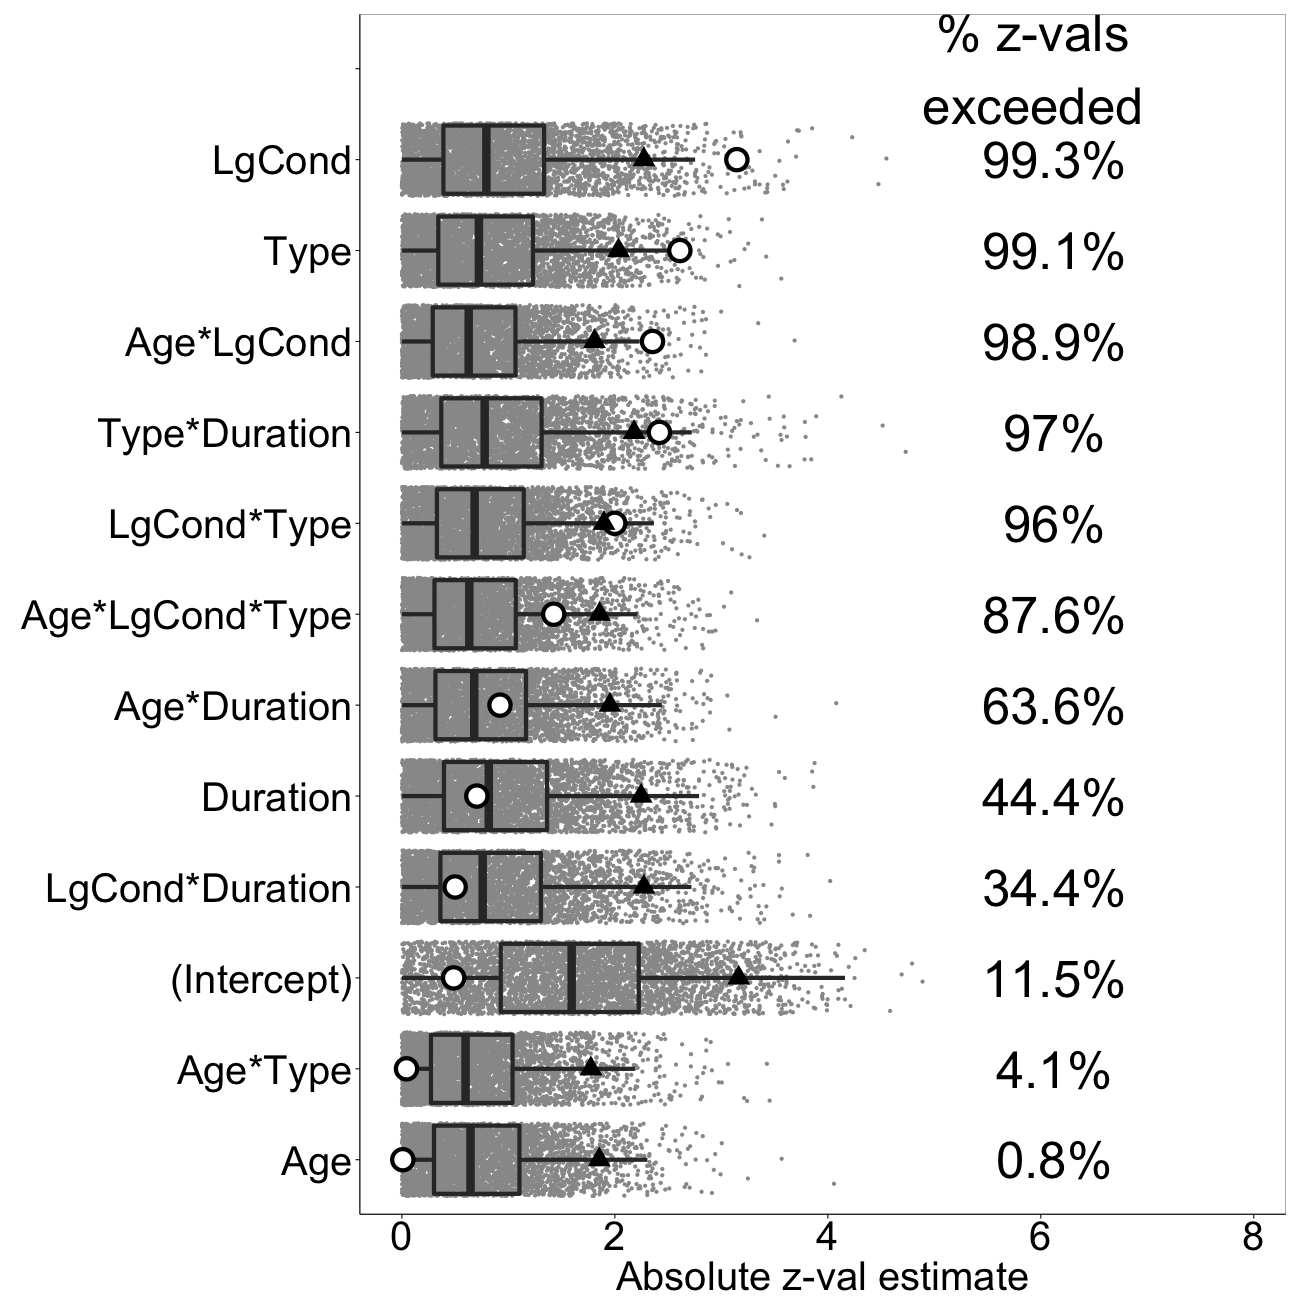
\includegraphics[width=0.44\textwidth]{figures/E1-chi-randrun-z-vals-absolute.png}\label{fig:E1-ChiTs}}
  \hfill
  \subfloat[Adults]{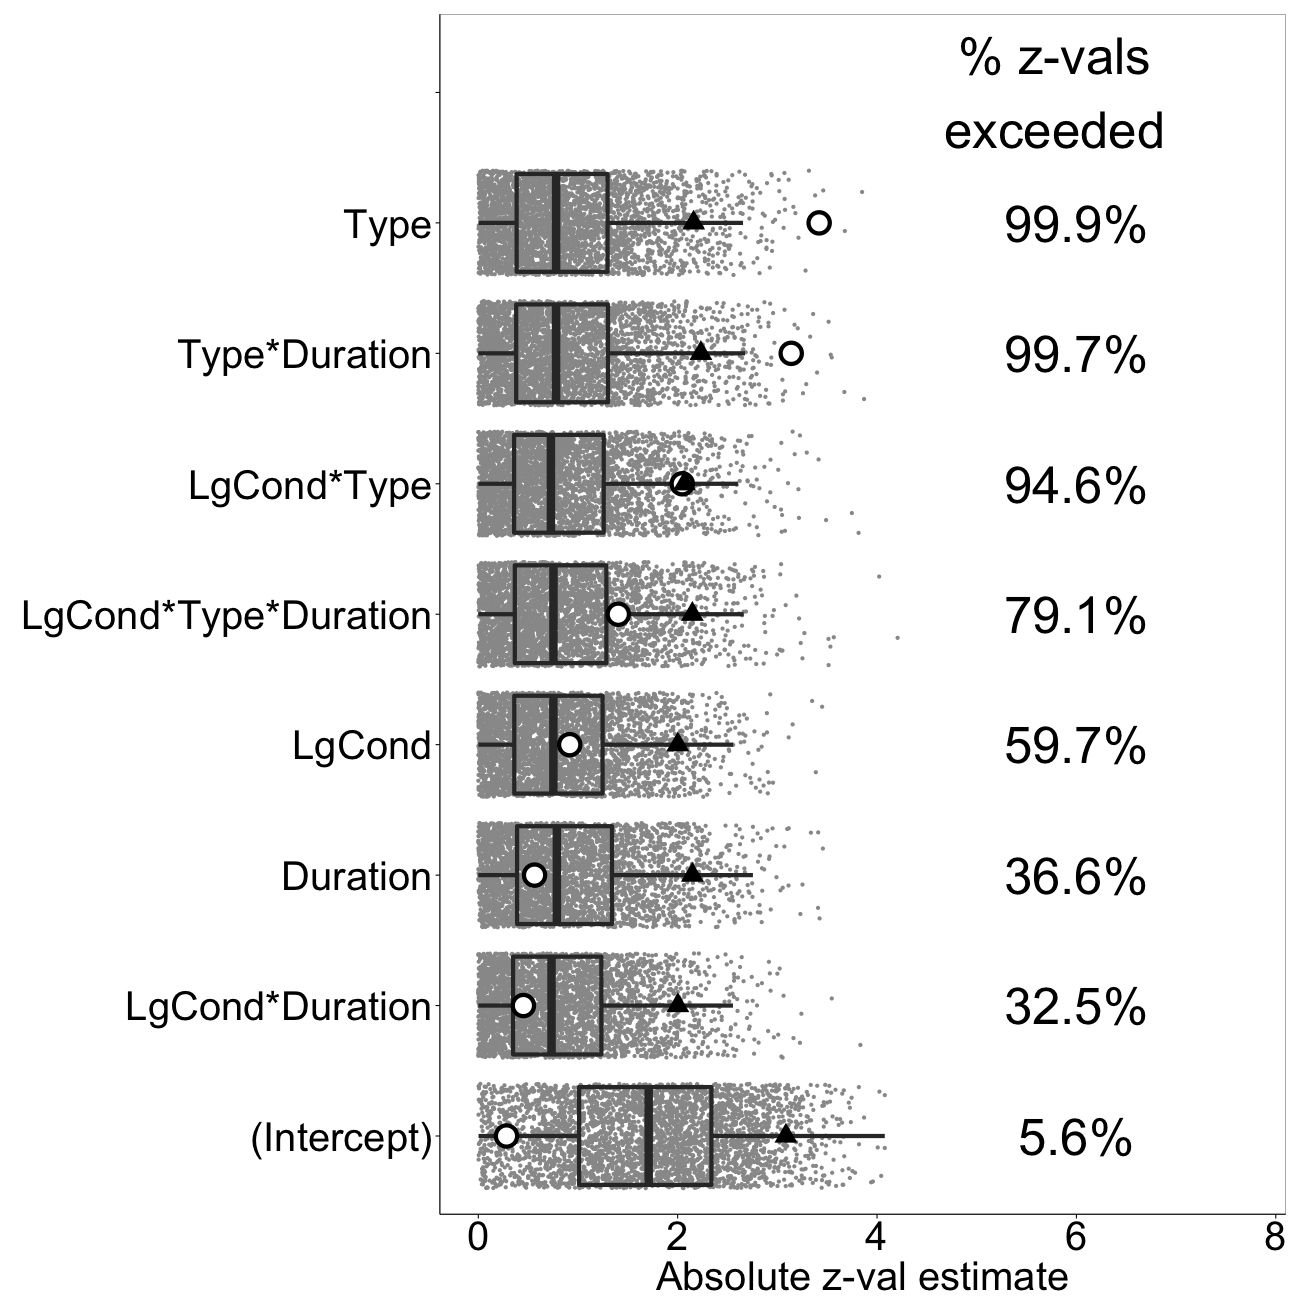
\includegraphics[width=0.44\textwidth]{figures/E1-adu-randrun-z-vals-absolute.png}\label{fig:E1-AduTs}}
  \caption{Random-permutation and original $|$\textit{z}-values$|$ for predictors of anticipatory gaze rates in Experiment 1.}
\label{fig:E1-Ts}
\end{sidewaysfigure}

\begin{sidewaysfigure}[!htb]
  \centering
  \textbf{Experiment 1: \textit{$\beta$} estimates}\par\medskip
  \subfloat[Children]{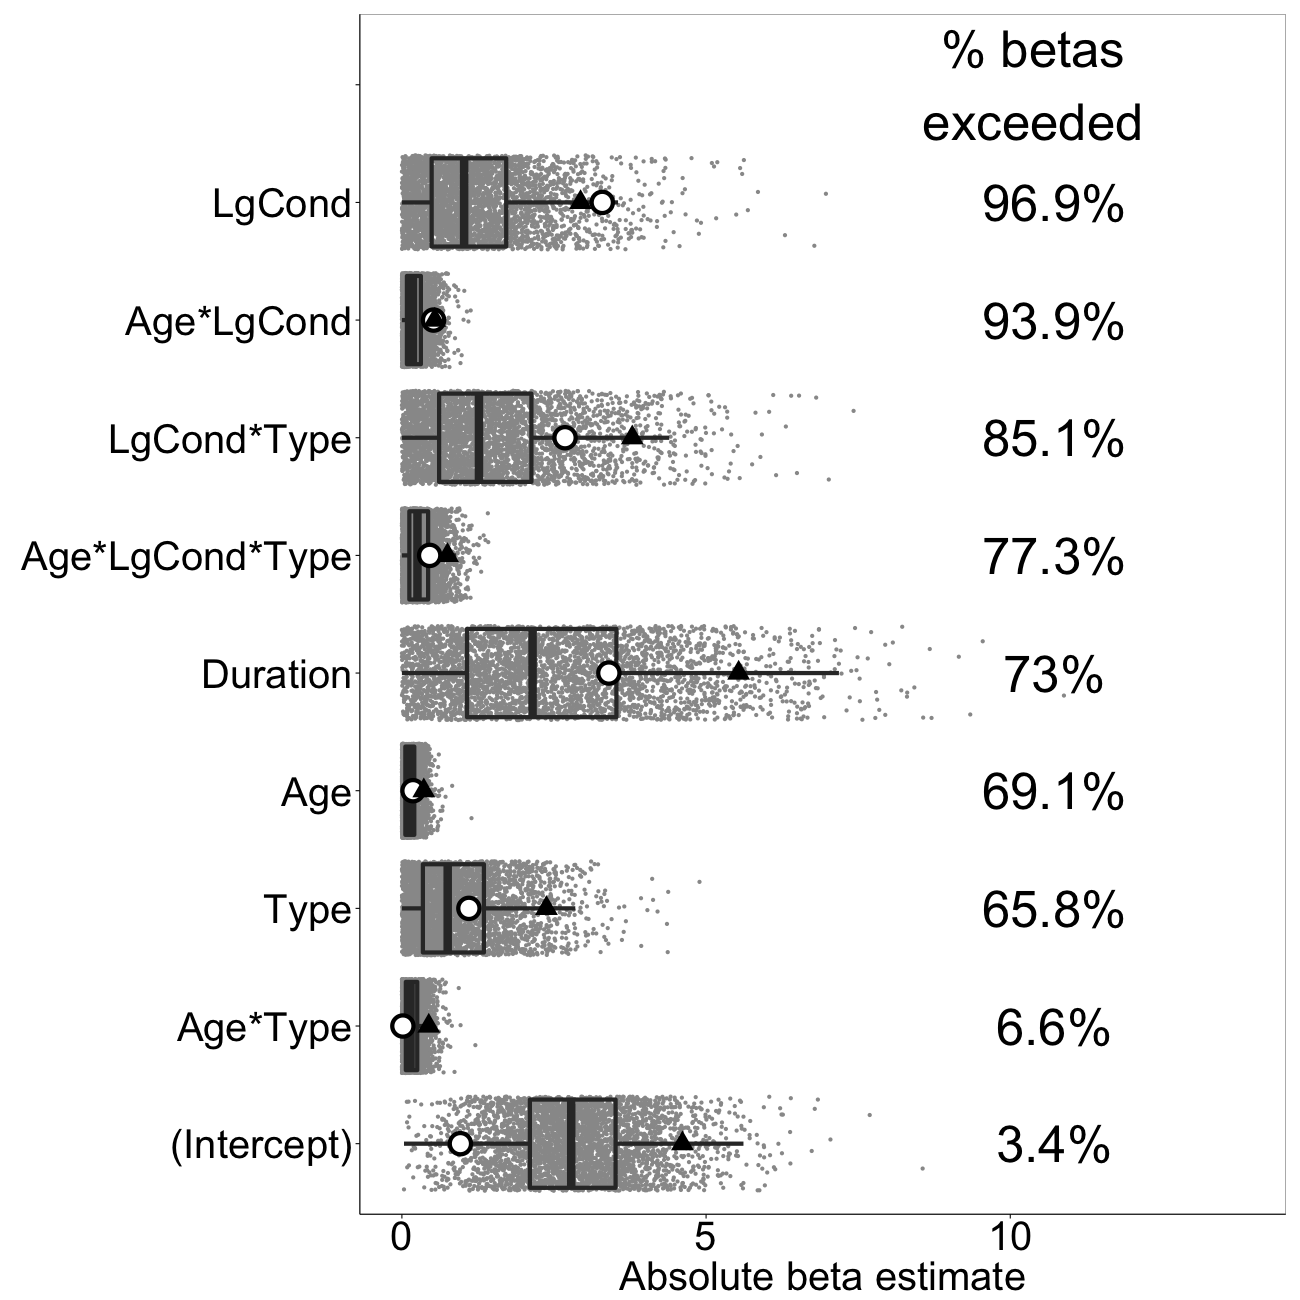
\includegraphics[width=0.44\textwidth]{figures/E1-chi-randrun-betas-absolute.png}\label{fig:E1-ChiBs}}
  \hfill
  \subfloat[Adults]{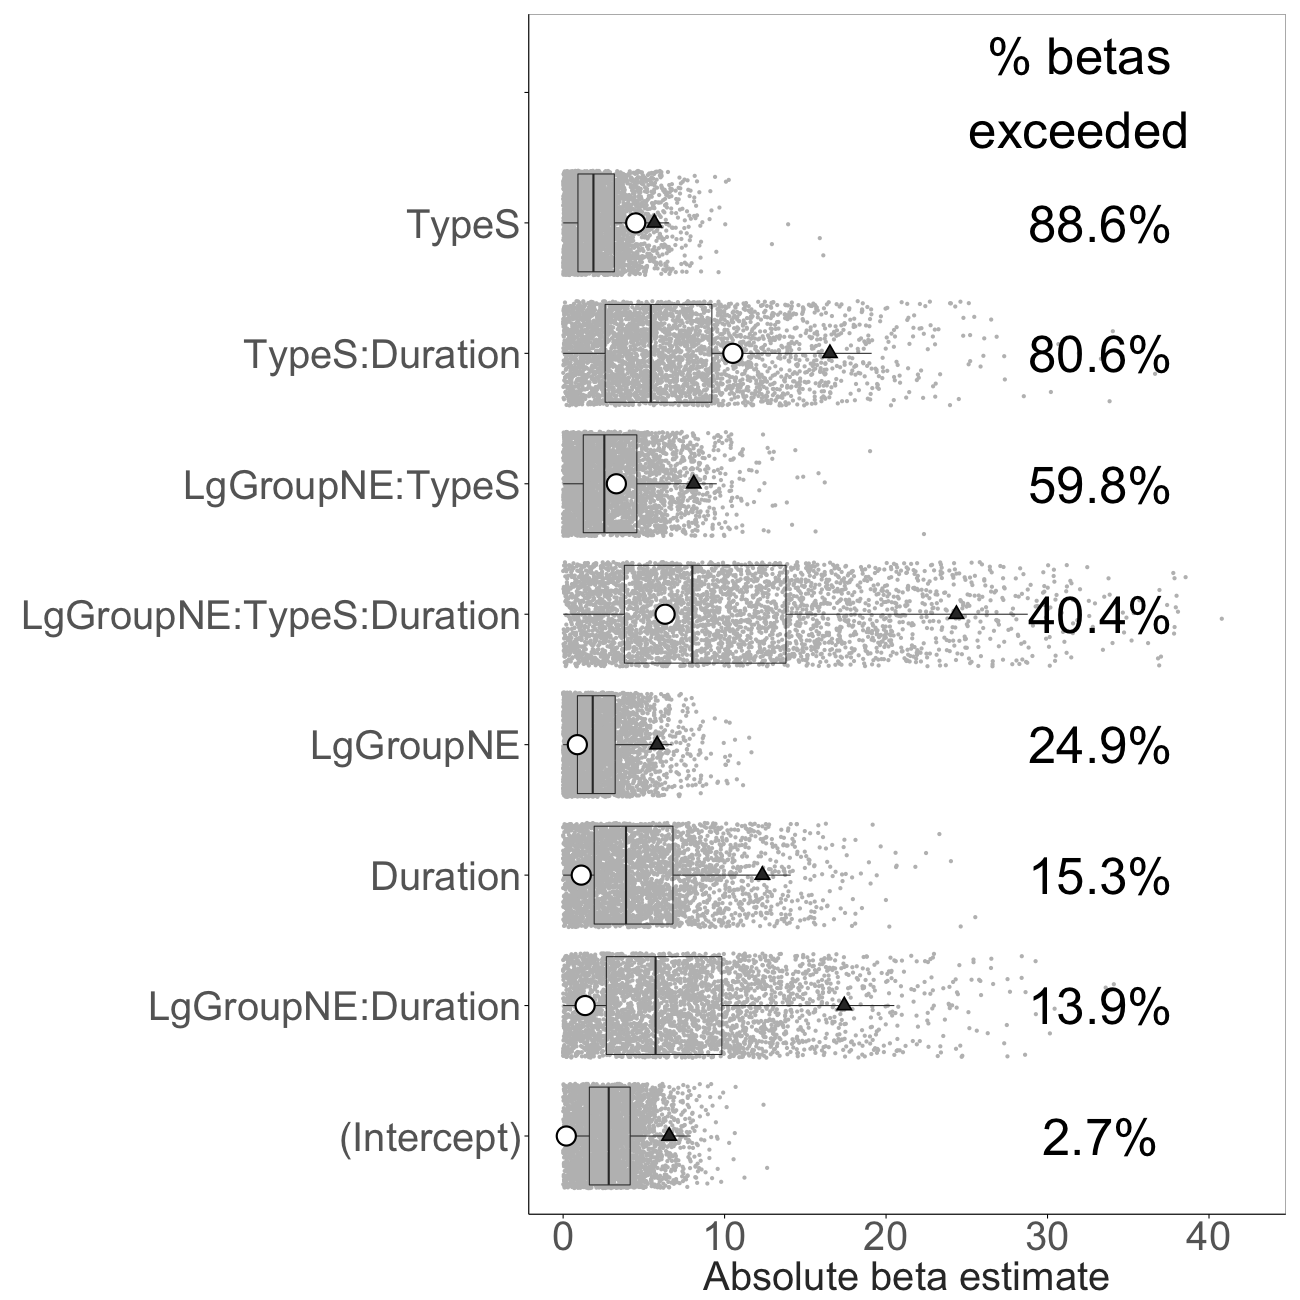
\includegraphics[width=0.44\textwidth]{figures/E1-adu-randrun-betas-absolute.png}\label{fig:E1-AduBs}}
  \caption{Random-permutation and original $|$\textit{$\beta$}-values$|$ for predictors of gaze rates in Experiment 1.}
\label{fig:E1-Bs}
\end{sidewaysfigure}

\begin{sidewaysfigure}[!htb]
  \centering
  \textbf{Experiment 1: \textit{SE} estimates}\par\medskip
  \subfloat[Children]{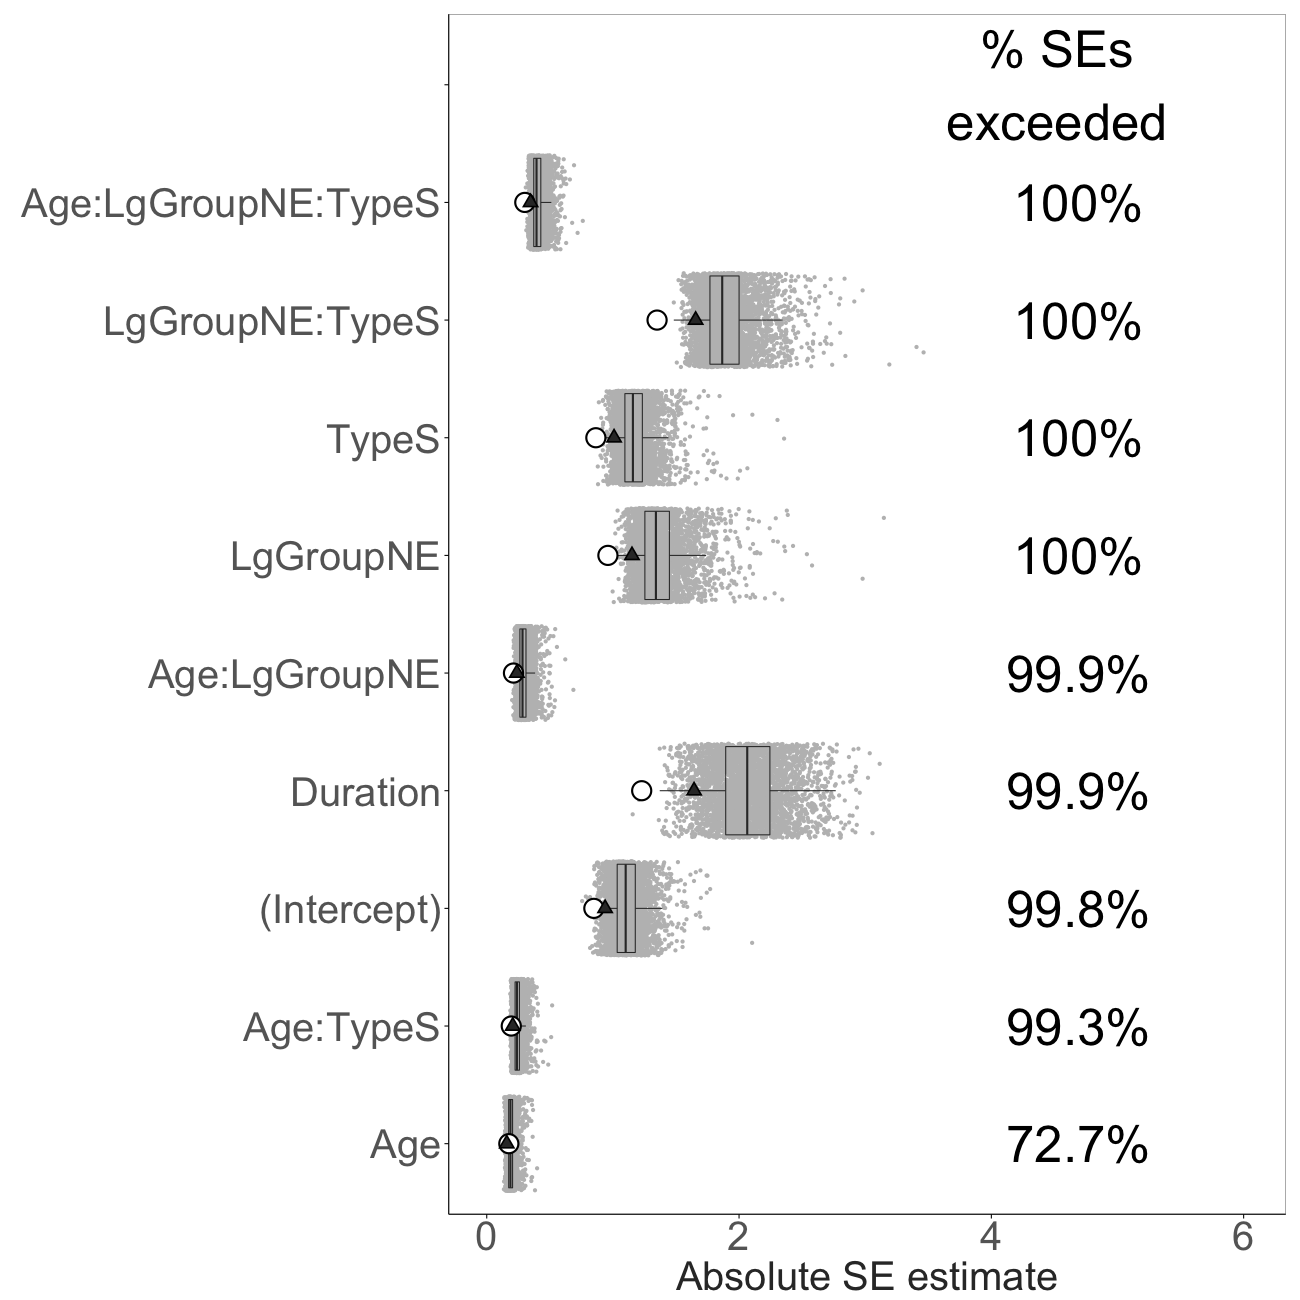
\includegraphics[width=0.44\textwidth]{figures/E1-chi-randrun-SEs-absolute.png}\label{fig:E1-ChiSEs}}
  \hfill
  \subfloat[Adults]{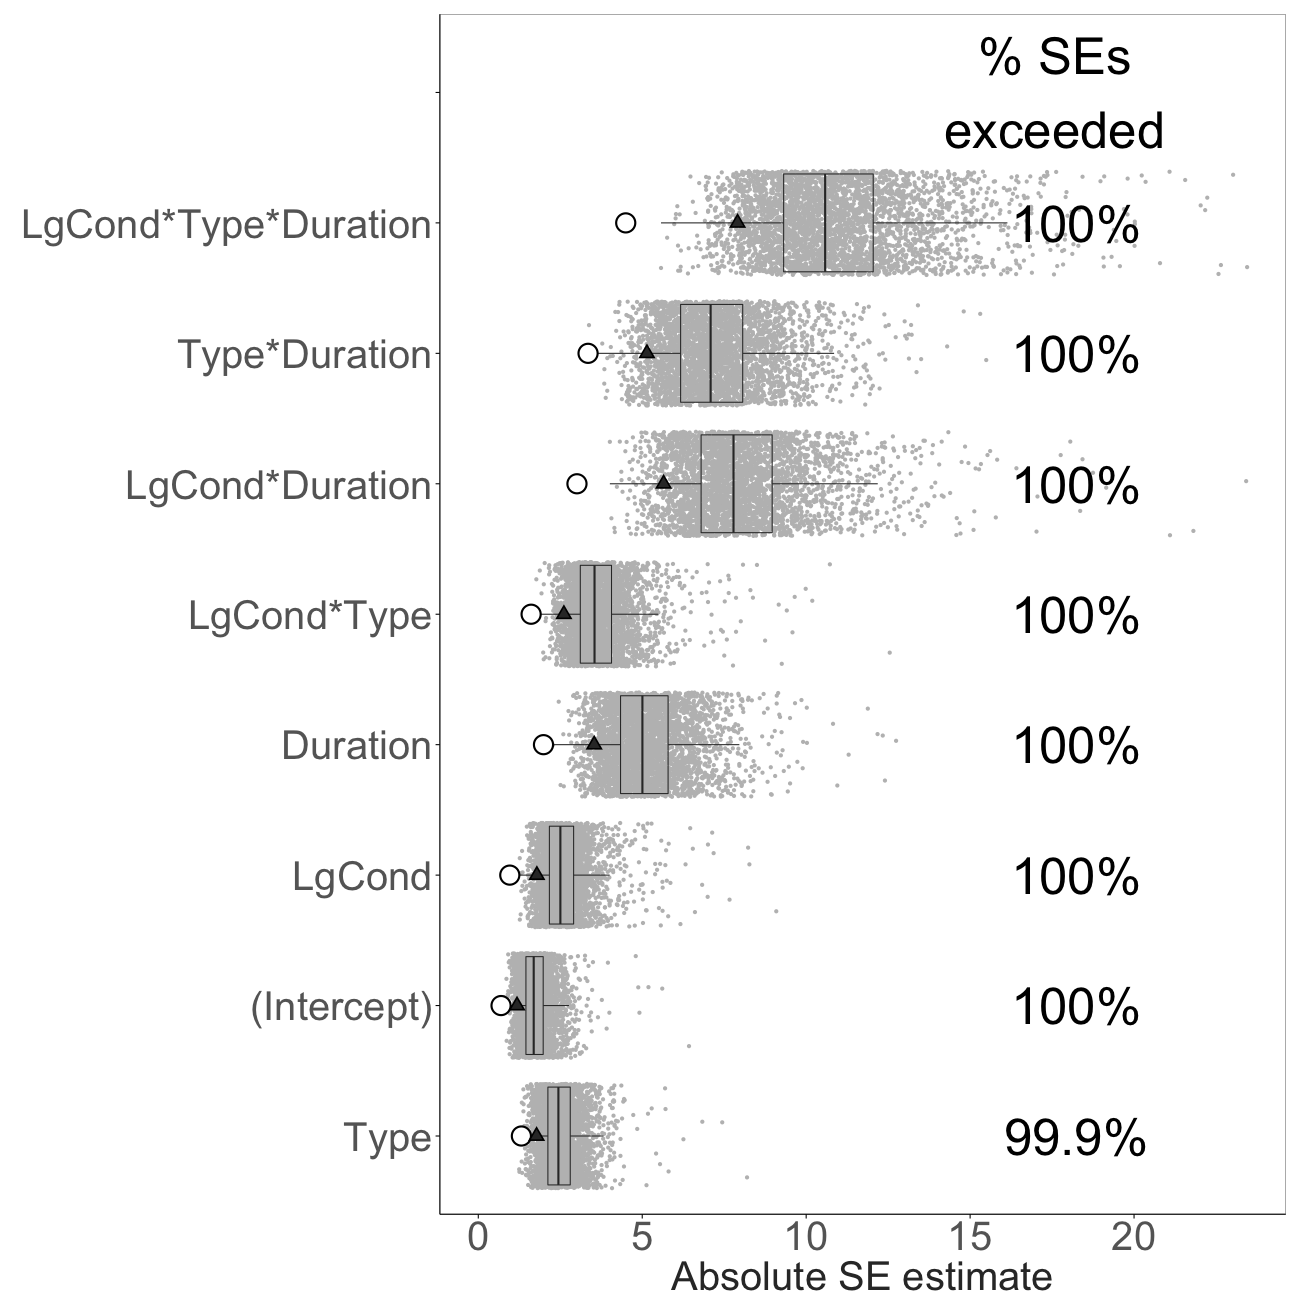
\includegraphics[width=0.44\textwidth]{figures/E1-adu-randrun-SEs-absolute.png}\label{fig:E1-AduSEs}}
  \caption{Random-permutation and original \textit{SE}-values for predictors of anticipatory gaze rates in Experiment 1.}
\label{fig:E1-SEs}
\end{sidewaysfigure}

\begin{sidewaysfigure}[!htb]
  \centering
  \textbf{Experiment 2: \textit{z} estimates}\par\medskip
  \subfloat[Children]{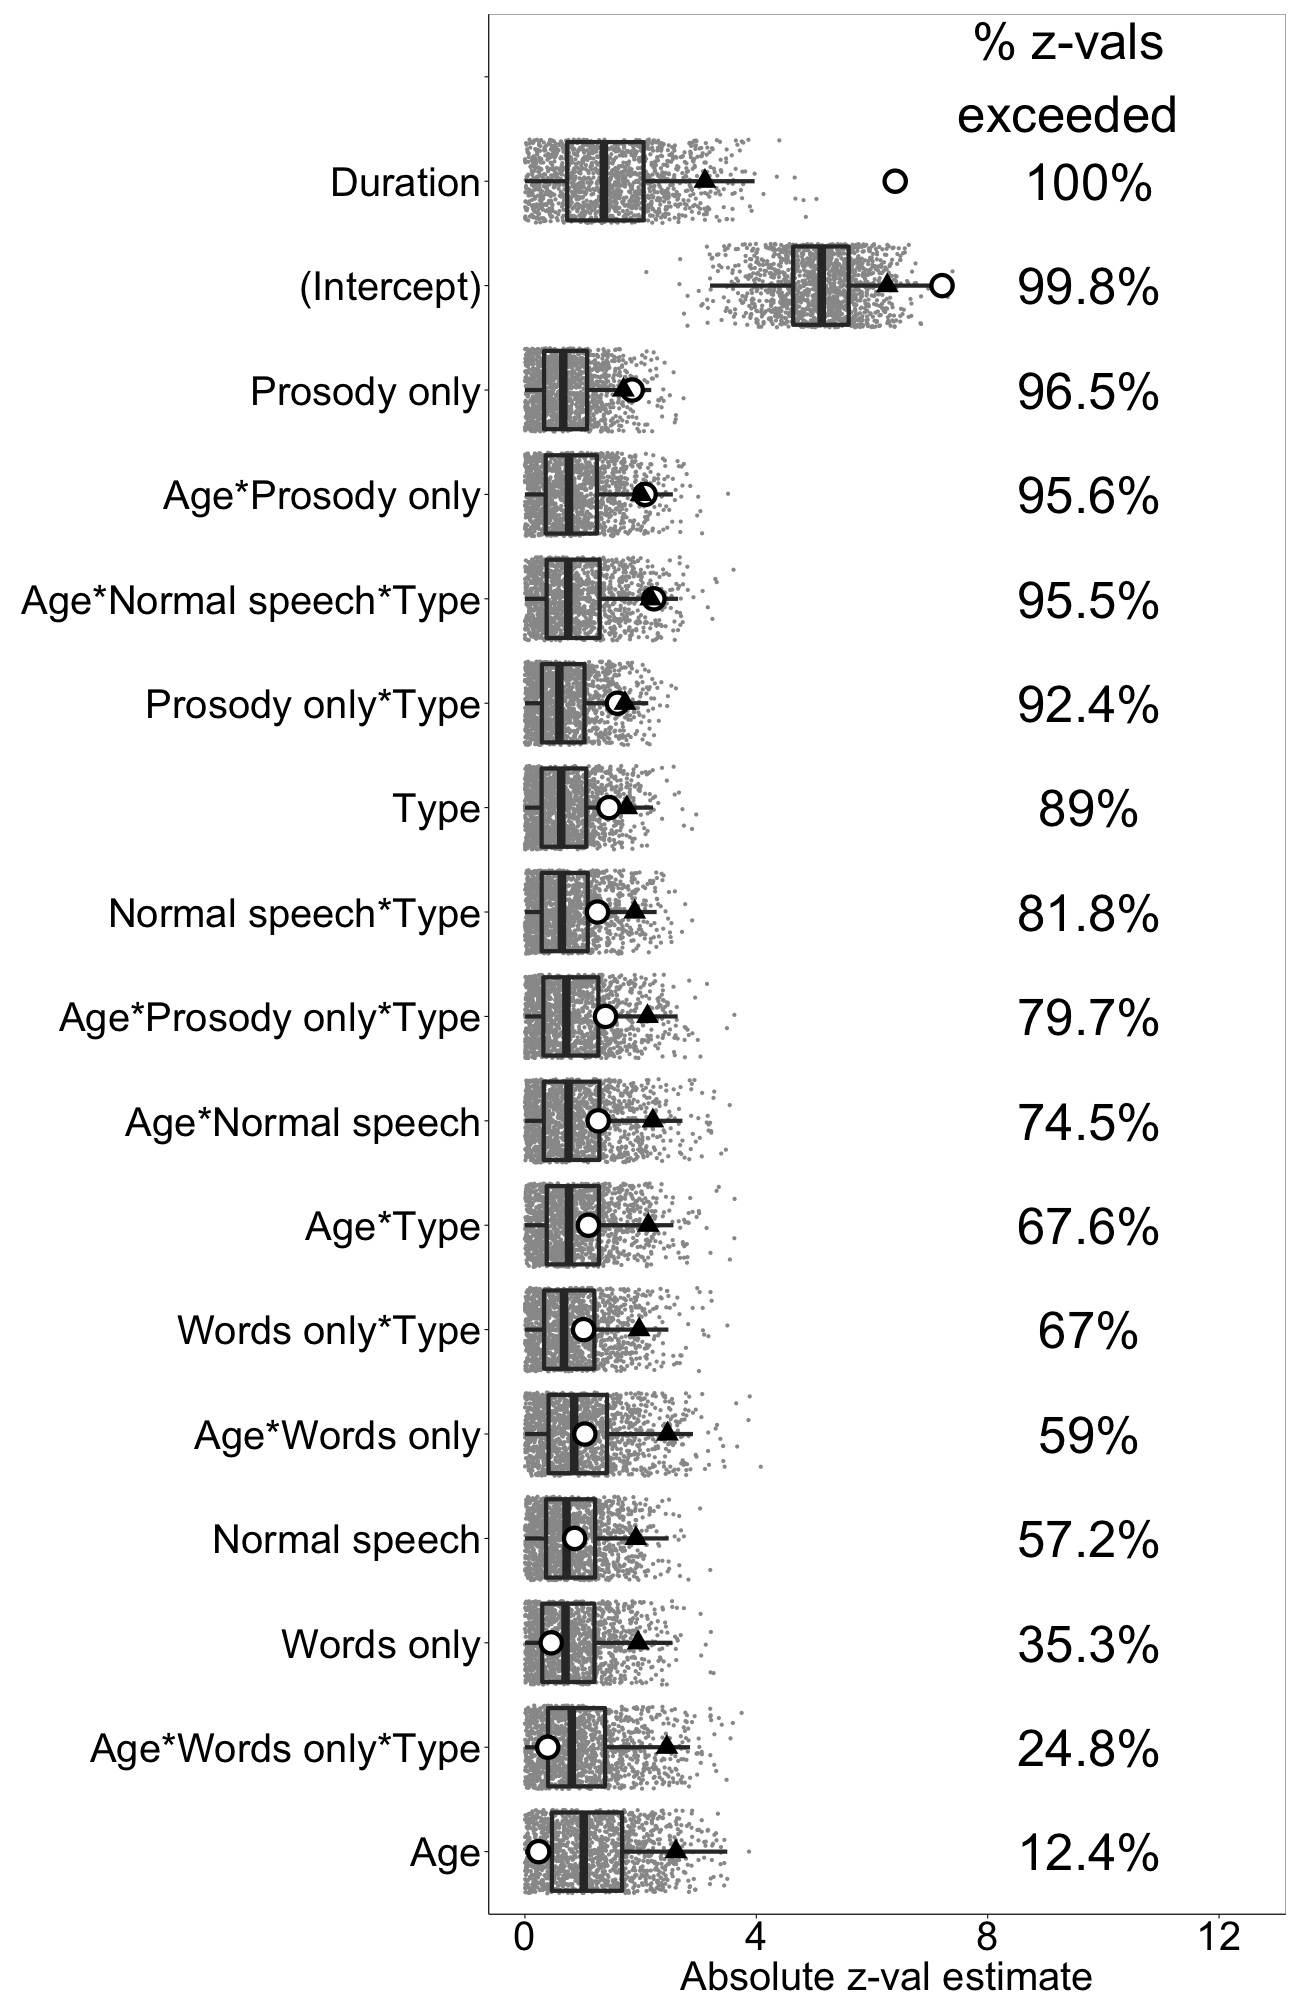
\includegraphics[width=0.44\textwidth]{figures/E2-chi-randrun-z-vals-absolute.png}\label{fig:E2-ChiTs}}
  \hfill
  \subfloat[Adults]{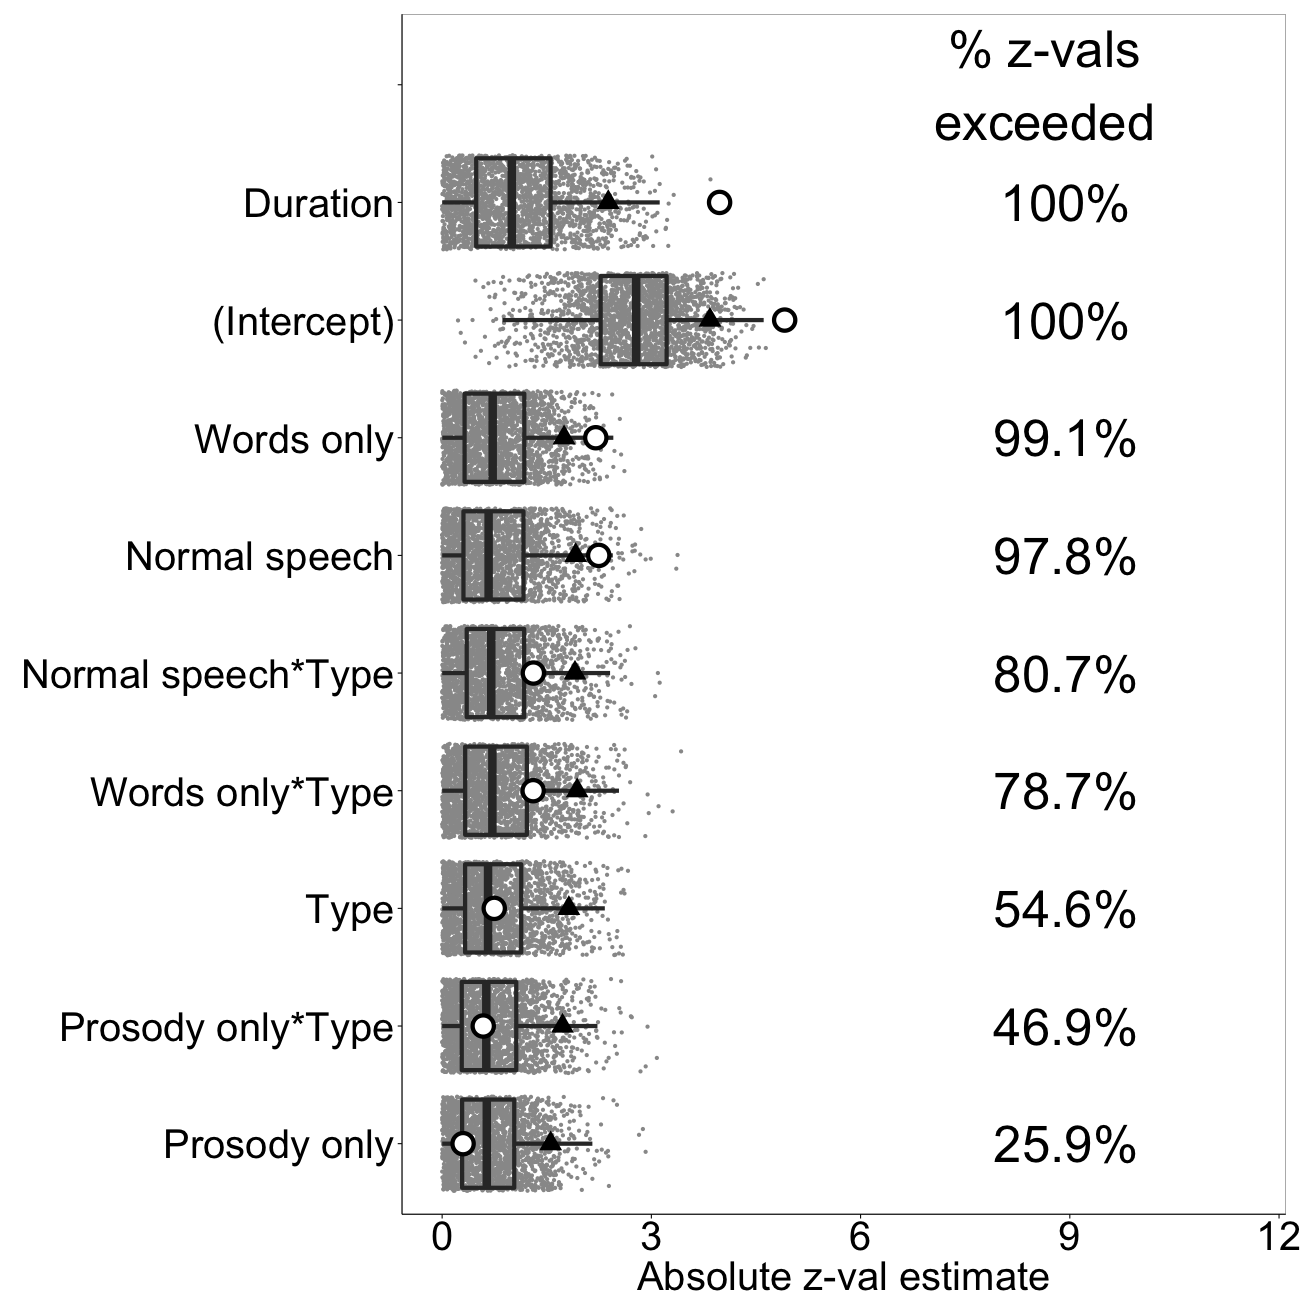
\includegraphics[width=0.44\textwidth]{figures/E2-adu-randrun-z-vals-absolute.png}\label{fig:E2-AduTs}}
  \caption{Random-permutation and original $|$\textit{z}-values$|$ for predictors of anticipatory gaze rates in Experiment 2.}
\label{fig:E2-Ts}
\end{sidewaysfigure}

\begin{sidewaysfigure}[!htb]
  \centering
  \textbf{Experiment 2: \textit{$\beta$} estimates}\par\medskip
  \subfloat[Children]{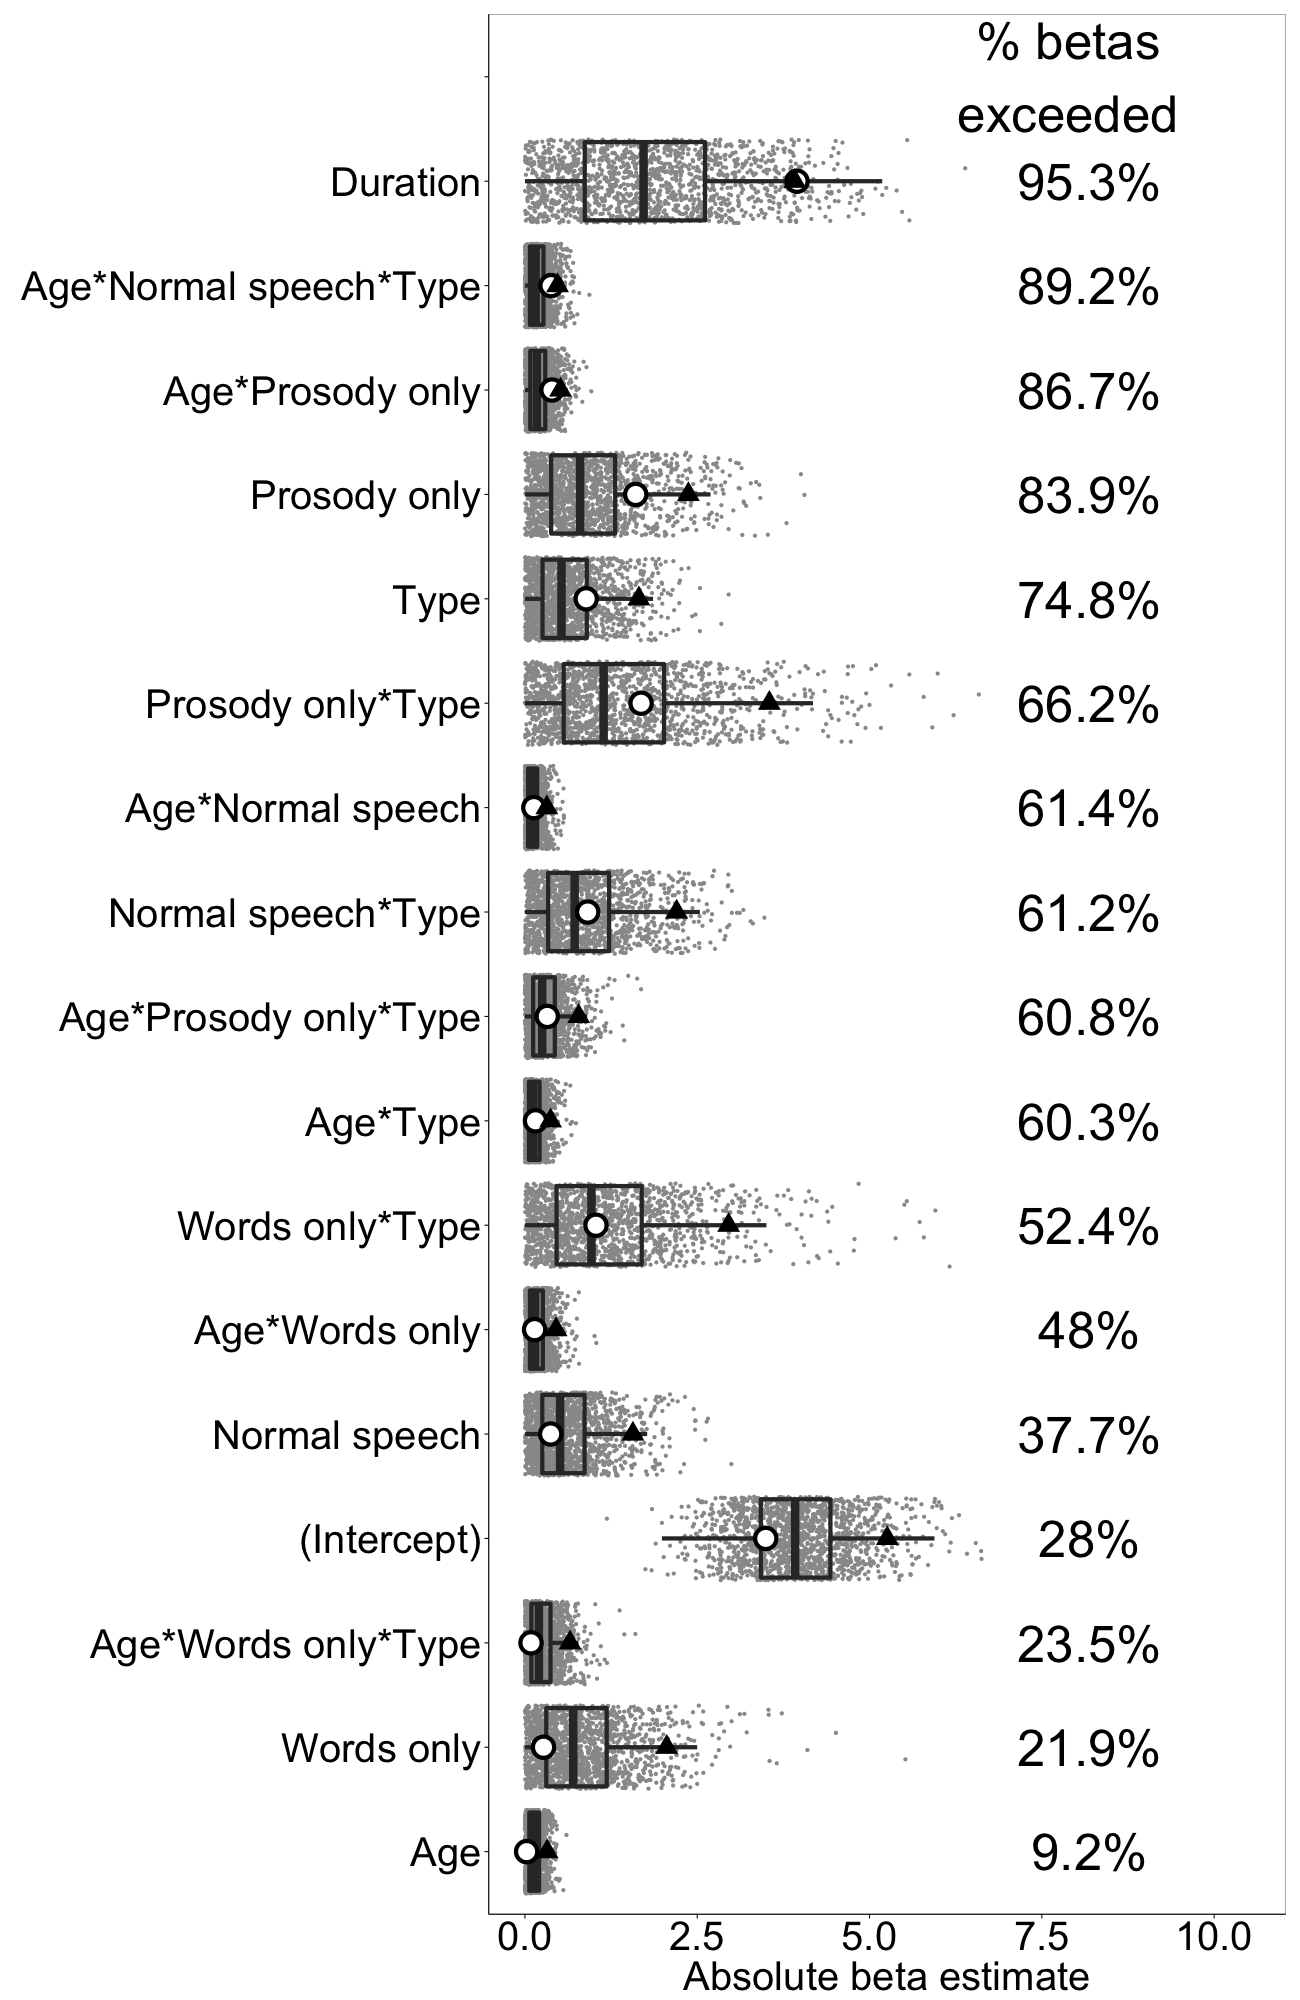
\includegraphics[width=0.44\textwidth]{figures/E2-chi-randrun-betas-absolute.png}\label{fig:E2-ChiBs}}
  \hfill
  \subfloat[Adults]{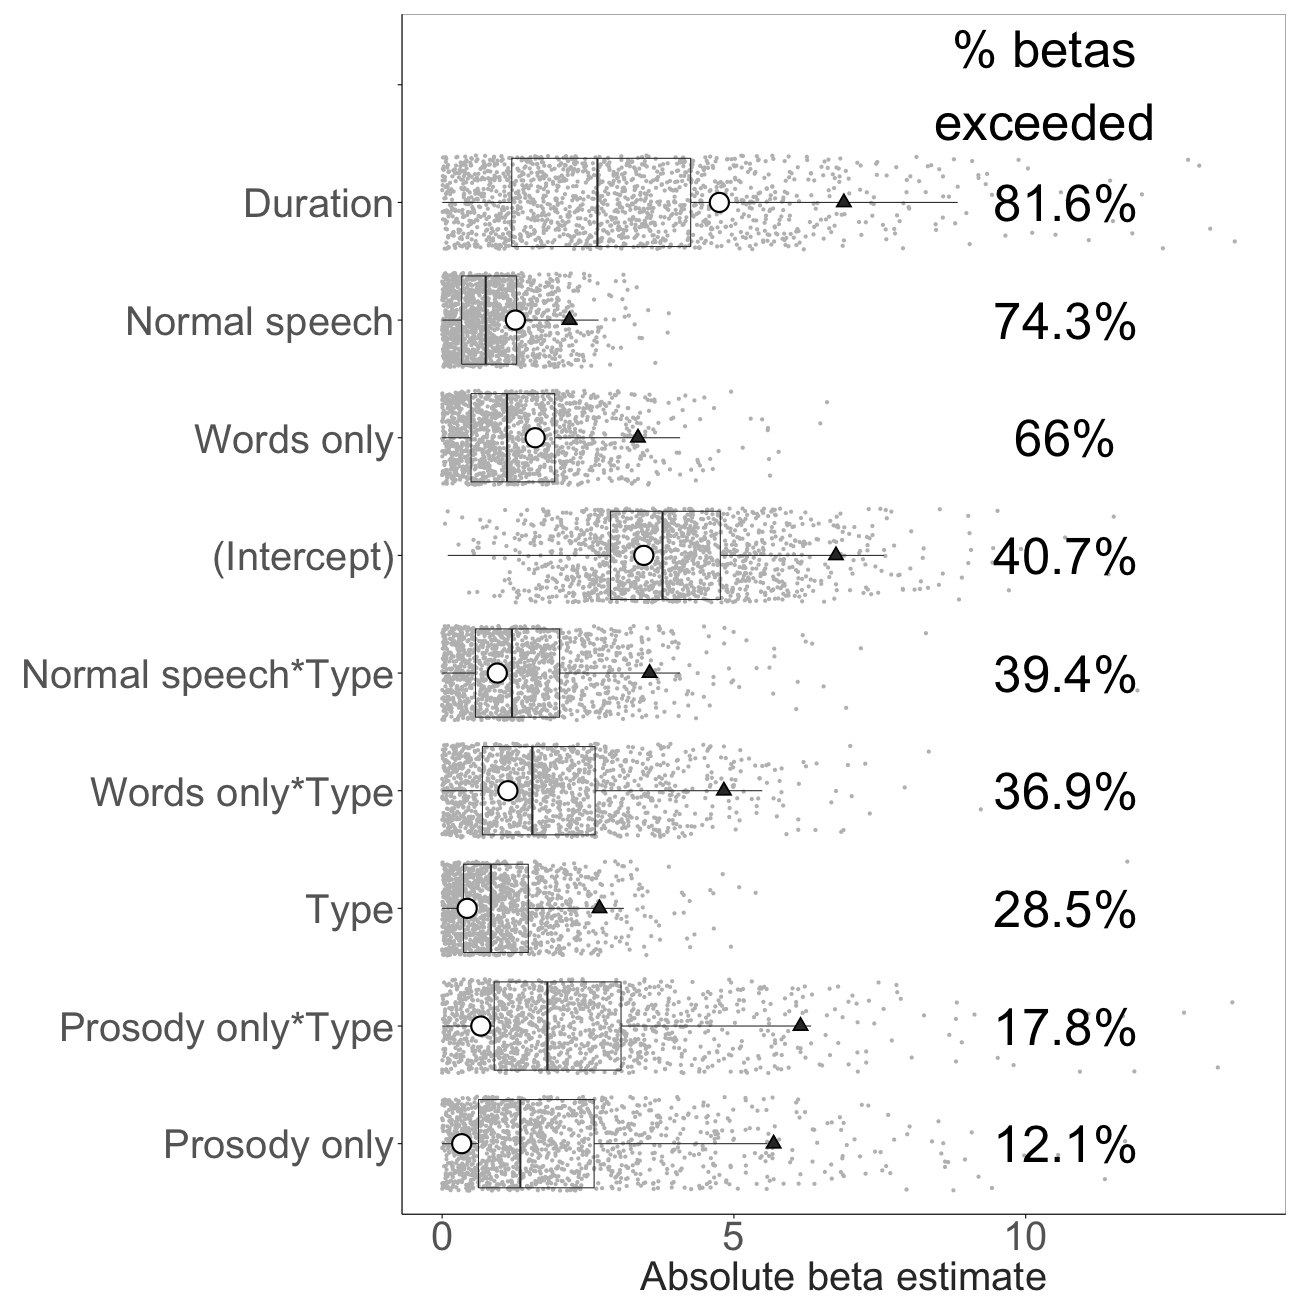
\includegraphics[width=0.44\textwidth]{figures/E2-adu-randrun-betas-absolute.png}\label{fig:E2-AduBs}}
  \caption{Random-permutation and original $|$\textit{$\beta$}-values$|$ for predictors of anticipatory gaze rates in Experiment 2.}
\label{fig:E2-Bs}
\end{sidewaysfigure}

\begin{sidewaysfigure}[!htb]
  \centering
  \textbf{Experiment 2: \textit{SE} estimates}\par\medskip
  \subfloat[Children]{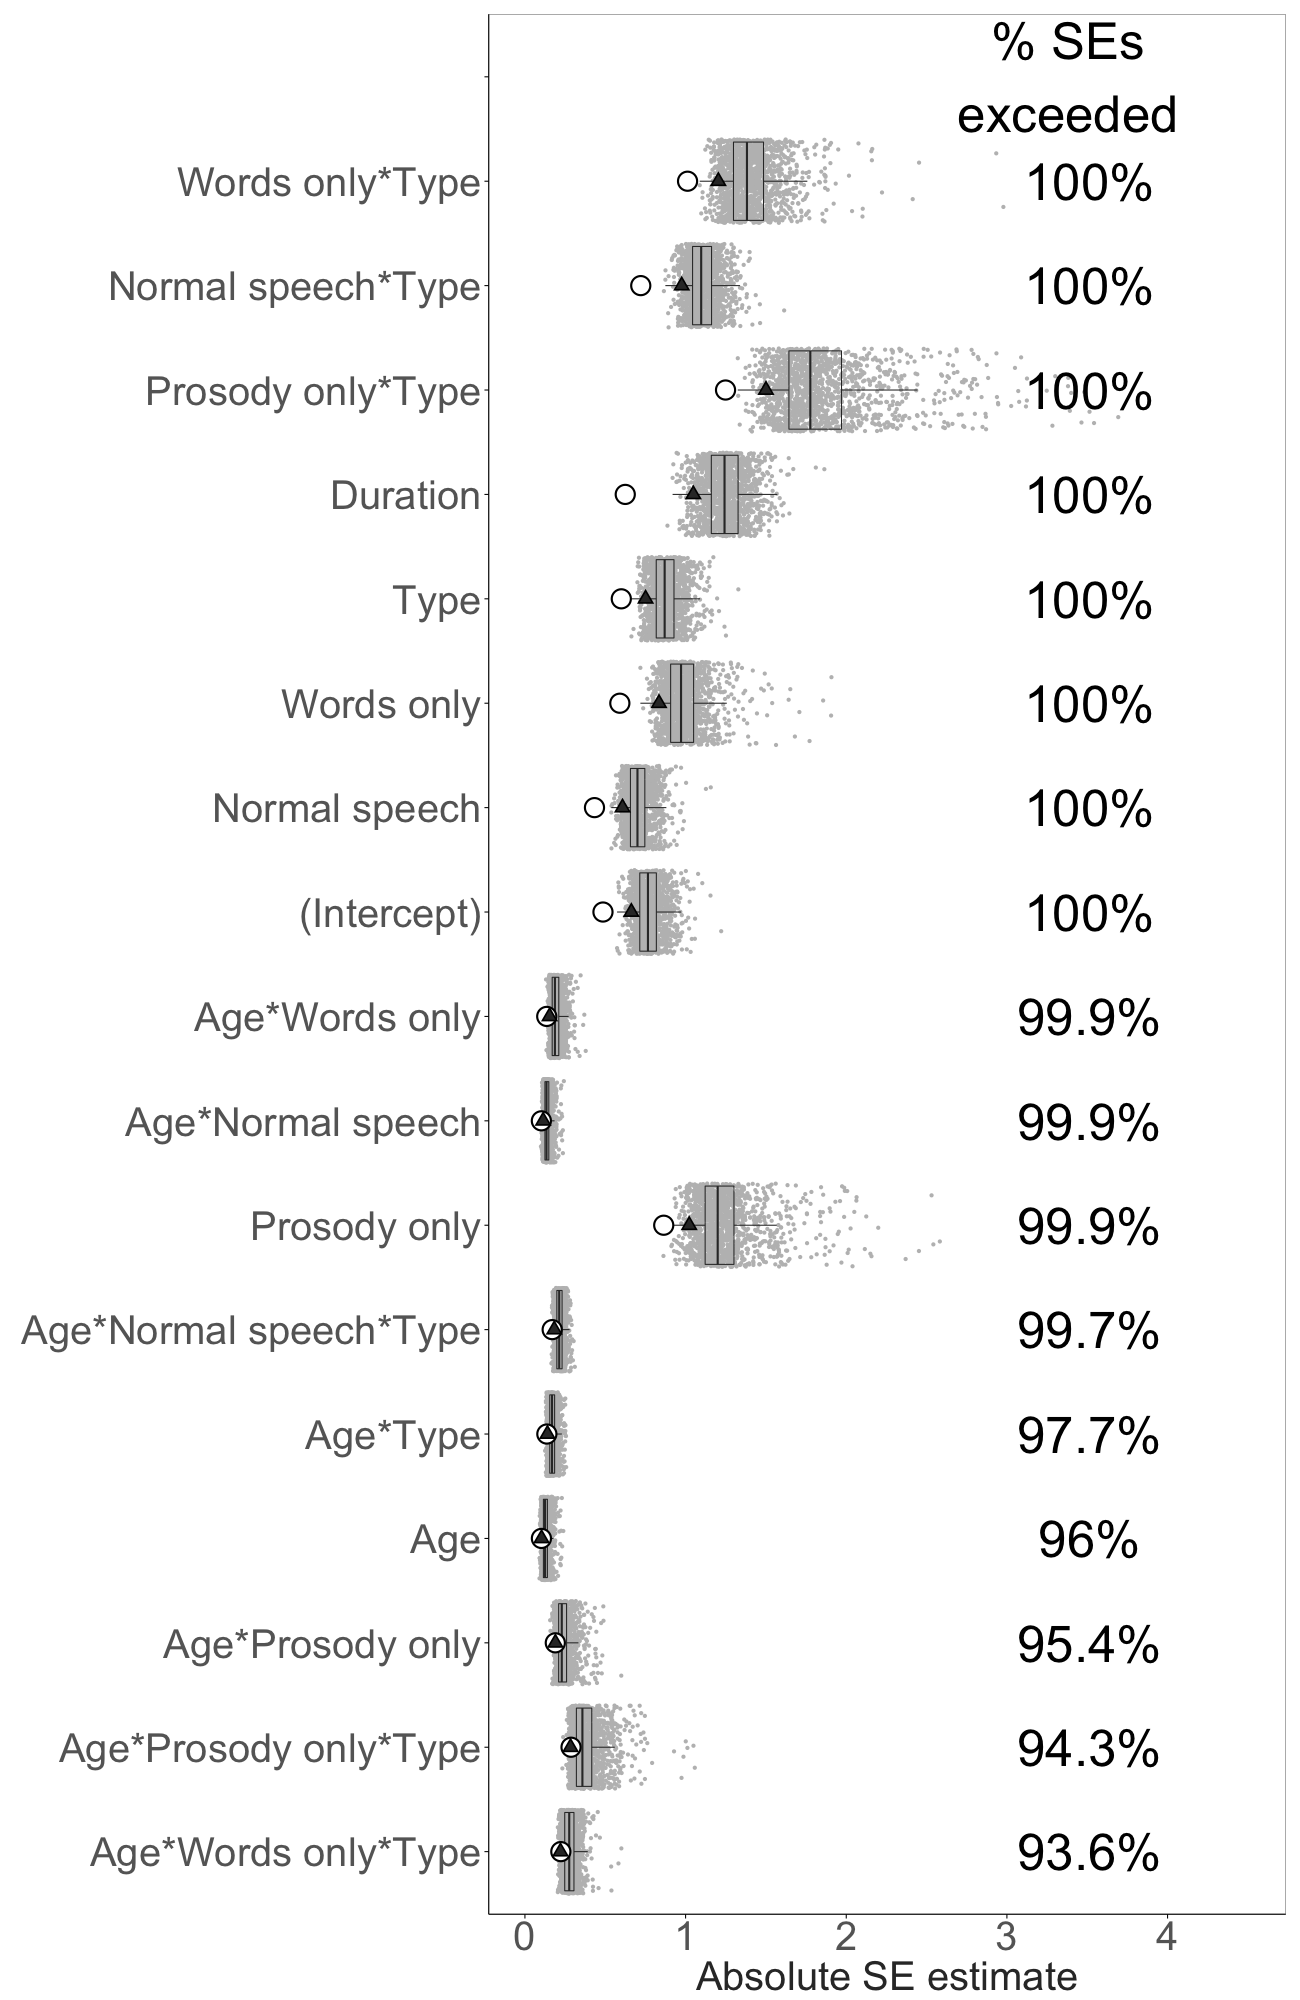
\includegraphics[width=0.44\textwidth]{figures/E2-chi-randrun-SEs-absolute.png}\label{fig:E2-ChiSEs}}
  \hfill
  \subfloat[Adults]{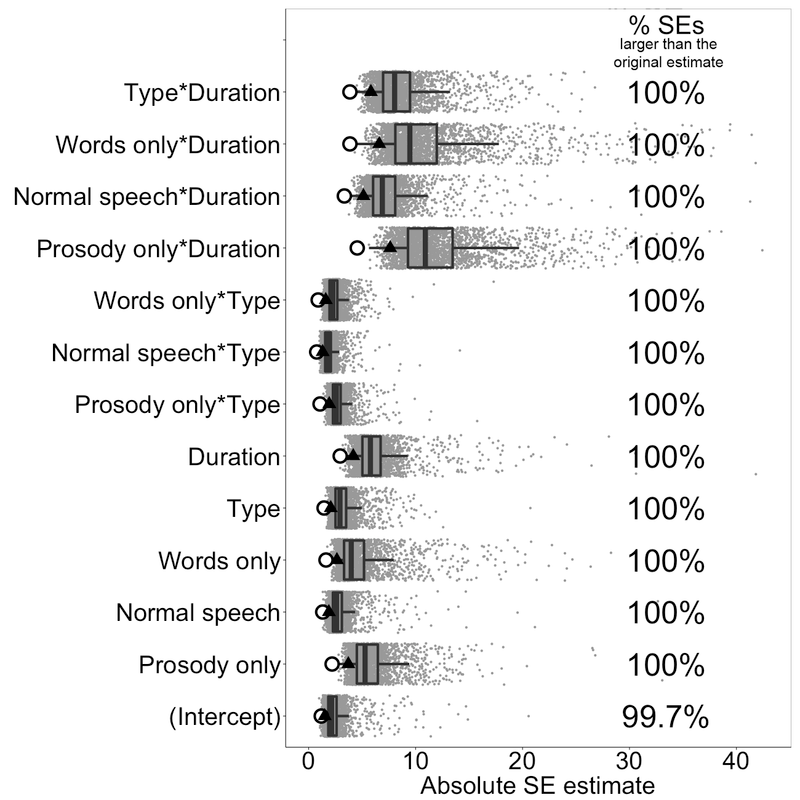
\includegraphics[width=0.44\textwidth]{figures/E2-adu-randrun-SEs-absolute.png}\label{fig:E2-AduSEs}}
  \caption{Random-permutation and original \textit{SE}-values for predictors of anticipatory gaze rates in Experiment 2.}
\label{fig:E2-SEs}
\end{sidewaysfigure}

\clearpage

\subsection{Non-convergent models}
In comparing the real and randomly permuted datasets, we excluded the output of random-permutation models that gave convergence warnings to remove erratic model estimates from our analyses. Non-convergent models made up 22.4--24.4\% of the random permutation models in Experiment 1 and 69--70\% of the random permutation models in Experiment 2. The \textit{z}-values for each predictor in the converging and non-converging models from Experiment 1 are shown in Table \ref{tab:nonconv_e1}.

Although many of the non-converging models show estimates within range of the converging models (e.g., with a mean difference of only 0.09 in median \textit{z}-value across predictors), they also show many radically outlying estimates (e.g., showing a mean difference of 237.3 in mean \textit{z}-value across predictors). Similar patterns were obtained in the non-converging models for Experiment 2 and persisted even when we tried other optimizers.

We suspect that the issue derives from data sparsity in some of the random permutations. This problem is known to occur when there are limited numbers of binary observations in each of a design matrix's bins \citep{allison2004}. We could instead use zero-inflated poisson or negative binomial regression models to allow for overdispersion in our data \citep{allison2012}. However, these would give us baselines for the normal, convergent model, which is not the aim of this analysis.

\linespread{1}
\begin{sidewaystable}[!htbp]
  \begin{scriptsize}
\centering
  \begin{tabular}{lllllllllll}
    & Mean$_{C}$ & Mean$_{NC}$ & Median$_{C}$ & Median$_{NC}$ & \textit{SD}$_{C}$ & \textit{SD}$_{NC}$ & Min$_{C}$ & Min$_{NC}$ & Max$_{C}$ & Max$_{NC}$ \\ 
    \hline
	\textbf{\textit{Children}} &&&&& \\
    \hline
    (Intercept)					& -2.52	& -458.42	& -2.54	& -2.86	& 0.87	& 1319.22	& -5.53	& -8185.36		& 0.41	& 0.97 \\
    Age								& -0.51	& -17.83	& -0.49	& -0.53	& 0.79	& 83.78		& -3.71	& -672.2		& 2.3		& 342.8 \\
    LgCond							& -0.53	& -109.91	& -0.55	& -0.63	& 0.93	& 564.42	& -3.93	& -4418.74		& 3.23	& 2296.19 \\
    Type							& -0.1	& -29.66	& -0.09	& -0.1	& 0.98	& 515.12	& -4.06	& -4383.92		& 3.36	& 3416.68 \\
    Duration						& 0.99	& 345.53	& 0.98	& 1.15	& 1.07	& 1323.13	& -2.44	& -5048.24		& 5.78	& 9985.16 \\
    Age*LgCond					& 0.19	& 10.64		& 0.2		& 0.18	& 0.9		& 109.6		& -3.31	& -581.61		& 3.59	& 946.81 \\
    Age*Type						& 0.02	& -1.8		& 0.001	& -0.04	& 0.9		& 98.27		& -3.36	& -884.36		& 3.45	& 640.43 \\
    LgCond*Type					& 0.2		& 45.32		& 0.2		& 0.27	& 0.96	& 691.3		& -3.12	& -4160.06		& 3.39	& 5107.64 \\
    Age*LgCond*Type			& -0.12	& -14.23	& -0.12	& -0.15	& 0.93	& 156.72	& -2.98	& -1318.26		& 2.90	& 927.69 \\
    \hline
	\textbf{\textit{Adults}} &&&&& \\
    \hline
    (Intercept)    			& -1.63	& -126.14	& -1.71	& -1.73	& 0.97	& 713.39	& -4.08	& -12111.22	& 2.15	& 649.55		\\
    LgCond  						& -0.26	& -679.6	& -0.3	& -0.53	& 1.02	& 15894.33	& -3.45	& -494979.7	& 3.35	& 88581.58	\\
    Type 							& -0.11	& 6.29		& -0.13	& -0.04	& 1.11	& 501.5		& -3.85	& -6420.75		& 3.28	& 8177.88		\\
    Duration  					& 0.25	& 84.09		& 0.27	& 0.26	& 1.1		& 1152.94	& -3.25	& -10864.51	& 3.46	& 18540.62	\\
    LgCond*Type  				& 0.12	& -242.27	& 0.1		& 0.34	& 1.07	& 26836.7	& -3.41	& -622642.7	& 3.81	& 509198.4	\\
    LgCond*Duration			& 0.15	& 780.03	& 0.16	& 0.39	& 1.04	& 44105.02	& -3.84	& -798498.6	& 3.55	& 1145951	\\
    Type*Duration 				& 0.05	& -6.56		& 0.05	& 0.02	& 1.13	& 1389.9	& -3.54	& -15979.22	& 3.87	& 16419.46	\\
    LgCond*Type*Duration	& -0.06	& 1083.63	& -0.08	& -0.21	& 1.1		& 63116.54	& -4.21	& -1201895		& 4.02	& 1284965	\\
    \hline
  \end{tabular}
  \caption{Estimated \textit{z}-values for each predictor in converging (\textit{C}) and non-converging (\textit{NC}) child and adult models from Experiment 1. }
\label{tab:nonconv_e1}
 \end{scriptsize}
\end{sidewaystable}
\linespread{2}

\section{Pairwise developmental tests}
\label{sec:pairwisedev}
\setcounter{figure}{0}
Experiments 1 and 2 both showed effects of age in interaction with linguistic condition and transition type (e.g., English vs. non-English). To explore these effects in more depth, we recorded the average difference score for the predictor that interacted with age for each participant (e.g., English minus non-English anticipatory switches), using these values to compute an average difference score over participants in each age group (e.g., age 3, 4, and 5) within each random permutation. That averaging process produces 5,000 baseline-derived difference scores for each age group.

We then made pairwise age comparisons of these difference scores (e.g., the linguistic condition effect in 3-year-olds vs. 4-year-olds), computing the percent of random-permutation difference scores exceeded by the real-data difference score. If the real-data difference score exceeded 95\% of the random-data age difference scores, we deemed it to be an age effect significantly different from chance---e.g., a significant difference between ages three and four in the effect of linguistic condition. This procedure is essentially a two-tailed \textit{t}-test, adapted for use with the randomly permuted baseline data.

In each of the plots below, the black dot represents the real data value for the effect being shown. The effect sizes from the 5,000 randomly permuted data sets are shown in the distribution. The percentage displayed is the percentage of random permutation values exceeded by the original data value (taking the absolute value of all data points for a two-tailed test). Comparisons marked with 95\% or higher are significant at the \textit{p}$<$0.05 level. 

\begin{sidewaysfigure}[!htb]
\begin{center}
\textbf{Experiment 1: Age and linguistic condition}\par\medskip
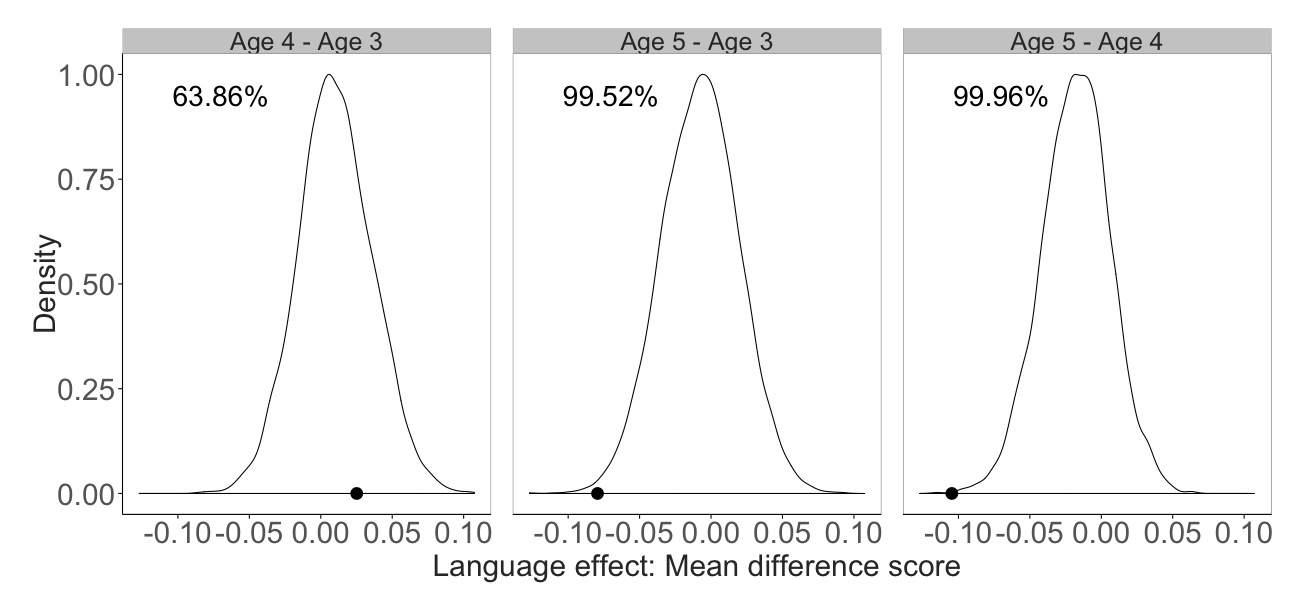
\includegraphics[width=0.95\textwidth]{figures/E1-child-randvsreal-ttest-agebylg.png}
\end{center}
\caption{Pairwise comparisons of the language condition effect across ages in Experiment 1.} 
\label{fig:E1-lgageinteraction}
\end{sidewaysfigure}

\begin{sidewaysfigure}[!htb]
\begin{center}
\textbf{Experiment 2: Age and the \textit{prosody only} condition}\par\medskip
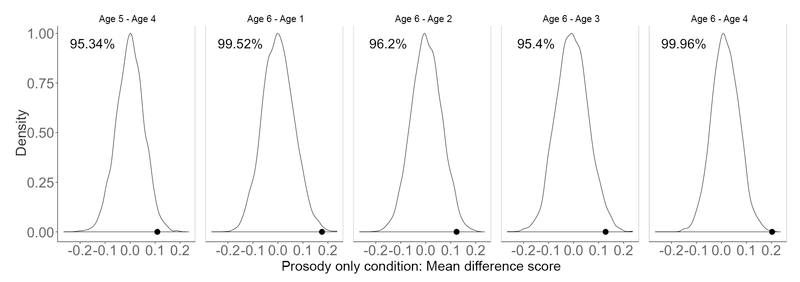
\includegraphics[width=0.95\textwidth]{figures/E2-child-randvsreal-ttest-muffledages.png}
\end{center}
\caption{Significant pairwise comparisons of the \textit{prosody only}-\textit{no speech} linguisitic condition effect, across ages in Experiment 2} 
\label{fig:E2-lgageinteraction}
\end{sidewaysfigure}

\begin{sidewaysfigure}[!htb]
\begin{center}
\textbf{Experiment 2: Age, transition type, and \textit{normal} speech}\par\medskip
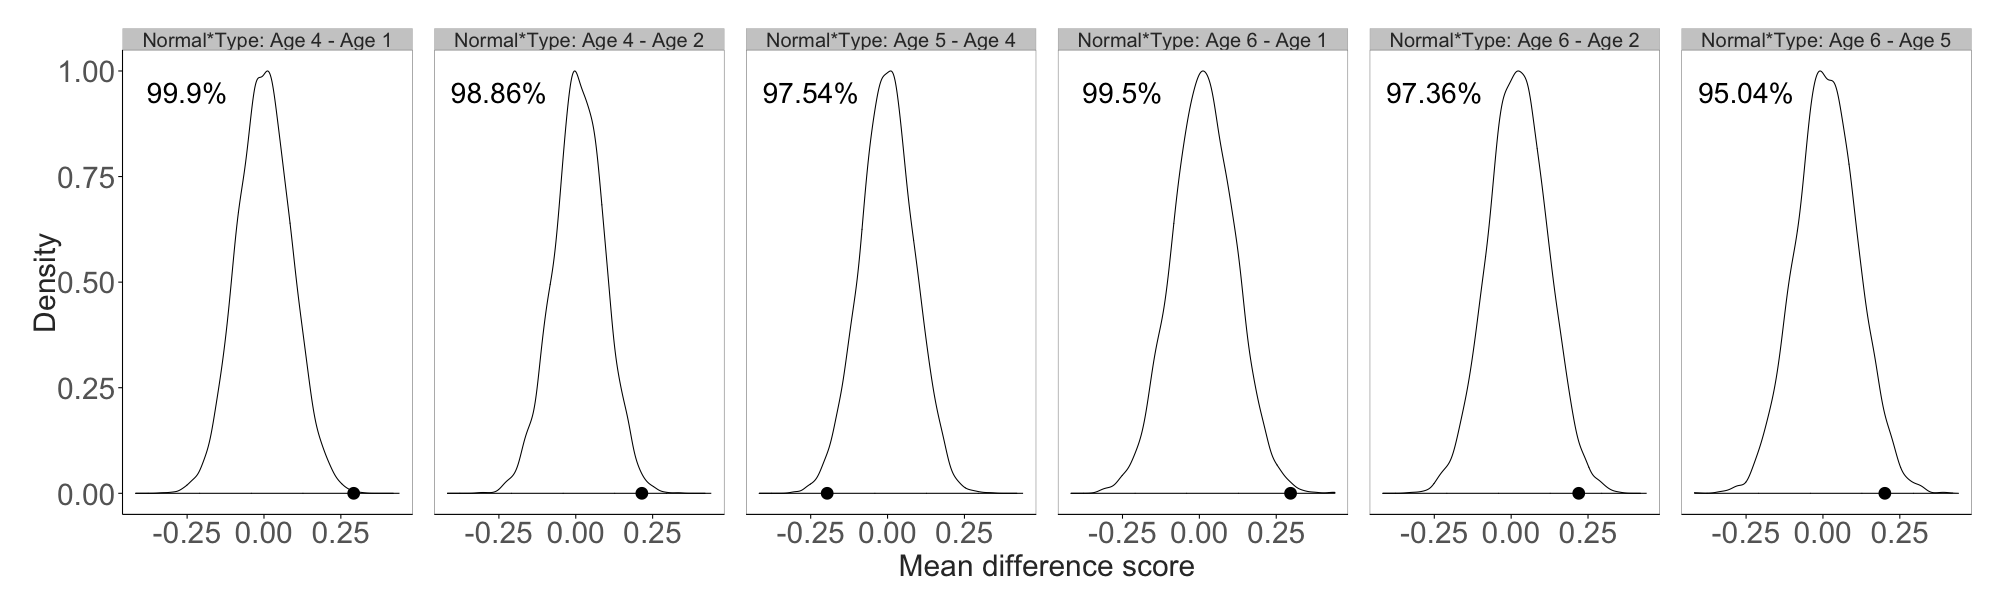
\includegraphics[width=0.95\textwidth]{figures/E2-child-randvsreal-ttest-normaltypesages.png}
\end{center}
\caption{Significant pairwise comparisons of the \textit{normal speech}-\textit{no speech} language condition effect for transition type, across ages, in Experiment 2.} 
\label{fig:E2-lgagetypeinteraction}
\end{sidewaysfigure}

\section{Boredom-driven anticipatory looking}
\label{sec:boredlooks}
\setcounter{figure}{0}  

One alternative hypothesis for children's anticipatory gazes is that they simply grow bored and start looking away at a constant rate after a turn begins. This data plotted here show a hypothetical group of boredom-driven participants (gray dots) compared to participants from the actual data in Experiment 2 (black dots). The hypothetical boredom-driven participants look away from the current speaker at a linear rate, beginning one second after the start of a turn. 

\begin{figure}[!htb]
\begin{center}
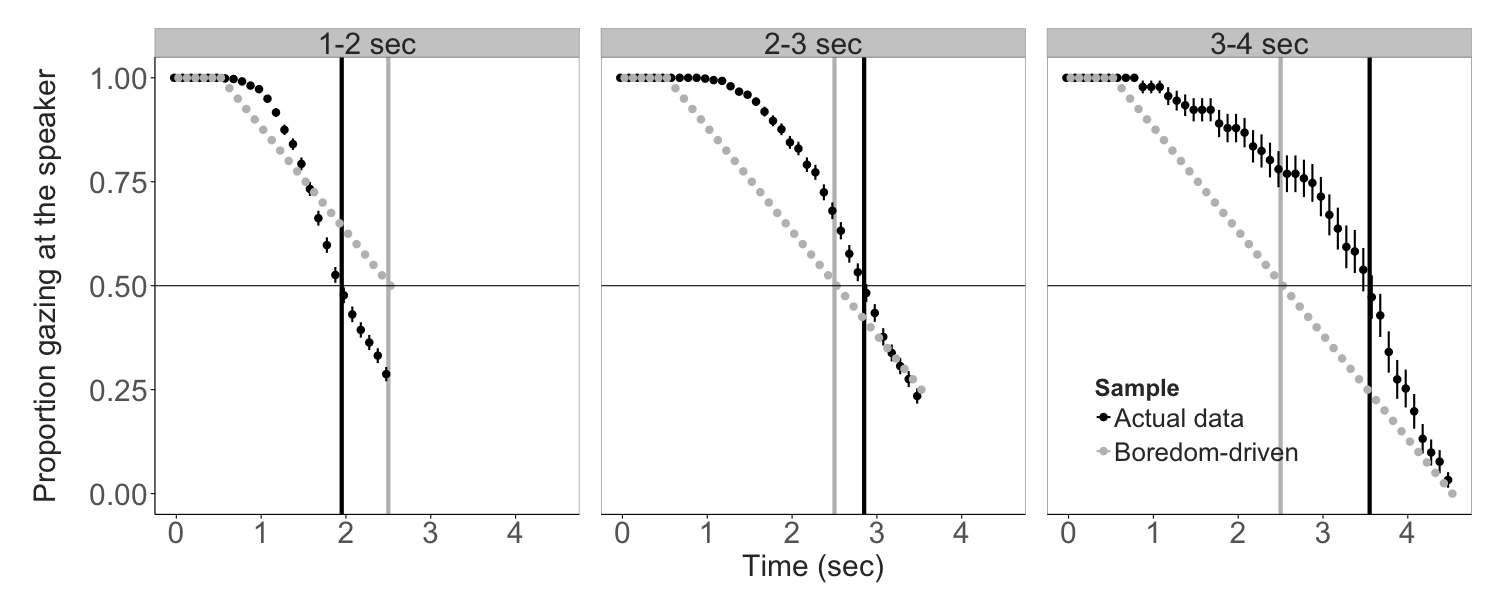
\includegraphics[width=0.95\textwidth]{figures/boredom-hypothesis.png}
\end{center}
\caption{Proportion of participants (hypothetical boredom-driven$=$gray; actual Experiment 2$=$black) looking at the current speaker, split by turn duration. Vertical bars indicate standard error in the experimental data.} 
\label{fig:boredomhypothesis}
\end{figure}

If children's switches away from the current speaker were driven by boredom, they would switch away equally quickly on long and short turns. However, as turn duration increased, children in the experiment looked at the current speaker for a longer period before looking away, suggesting that they were not switching away at a constant rate. We can see this pattern most clearly in the time at which 50\% of the children had switched away from the current (indicated by the horizontal line in Figure \ref{fig:boredomhypothesis}): children's gaze crossed this 50\% threshold at 2.0, 2.9, and 3.6 seconds after the start of speech for turns with durations of 1--2, 2--3, and 3--4 seconds, respectively. In contrast, the hypothetical boredom-driven children always hit the 50\% threshold at 2.5 seconds after the start of speech. This pattern suggests that, though children do look away with time, their looks away are not simply driven by boredom.

\clearpage

\section{Puppet pair and linguistic condition}
\label{sec:puppetconfound}
\setcounter{figure}{0}  
The design for Experiment 2 does not fully cross puppet pair (e.g., robots, blue puppets) with linguistic condition (e.g., \textit{words only} and \textit{no speech}). Even though each puppet pair is associated with different conversation clips across children (e.g., robots talking about kitties, birthday parties, and pancakes), the robot puppets themselves were exclusively associated with the \textit{words only} condition. Similarly, merpeople were exclusively associated with \textit{prosody only} speech, and the puppets wearing dressy clothes were exclusively associated with the \textit{no speech} condition. We designed the experiment this way to increase its pragmatic felicity for older children (i.e., robots make robot sounds, merpeople's voices are muffled under the water, the party-going puppets are in a `party' room with many other voices). There is therefore a confound between linguistic condition and puppet pair; for example, children could have made fewer anticipatory switches in the \textit{prosody only} condition because the puppets were less interesting. To test whether puppet pair drove the condition-based differences found in Experiment 2, we ran a short follow-up study.

\newpage
\noindent \textbf{Methods}
\medskip

\noindent We recruited 30 children between ages 3;0 and 5;11 from the Children's Discovery Museum of San Jose, California to participate in our experiment. All participants were native English speakers. Children were randomly assigned to one of six videos (five children per video).

\medskip
\noindent \textit{Materials}. We created 6 short videos from the stimulus recordings made for Experiment 2. Each video featured a puppet pair (red/blue/yellow/robot/ merpeople/party-goer; Figure \ref{fig:puppets}). Puppets in all six videos performed the exact same conversation recording (`birthday party'; Experiment 2) with normal, unmanipulated speech; this experiment therefore holds all things constant across stimuli except for the appearance of the puppets.
 
\medskip
\noindent \textit{Procedure}. We used the same experimental apparatus and procedure as in Experiments 1 and 2. Each participant was randomly assigned to watch only one of the six puppet videos. Five children watched each video. As in Experiment 2, the experimenter immediately began each session with calibration and then stimulus presentation because no special instructions were required. The entire experiment took less than three minutes.

\medskip
\noindent \textit{Data preparation}. We identified anticipatory gaze switches to the upcoming speaker using the same method as in Experiments 1 and 2.

\bigskip
\noindent \textbf{Results and discussion}
\medskip

\noindent We modeled children's anticipatory switches (yes or no at each transition) with mixed effects logistic regression, including puppet pair (robots/mer- people/party-goers/other-3) as a fixed effect and participant and turn transition as random effects. We grouped the red, blue, and yellow puppets together because they collectively represented the puppets used in the \textit{normal} speech condition---this follow-up experiment is meant to test whether the condition-based differences from Experiment 2 arose from the puppets used in each condition.

\begin{figure}[!htb]
\begin{center}
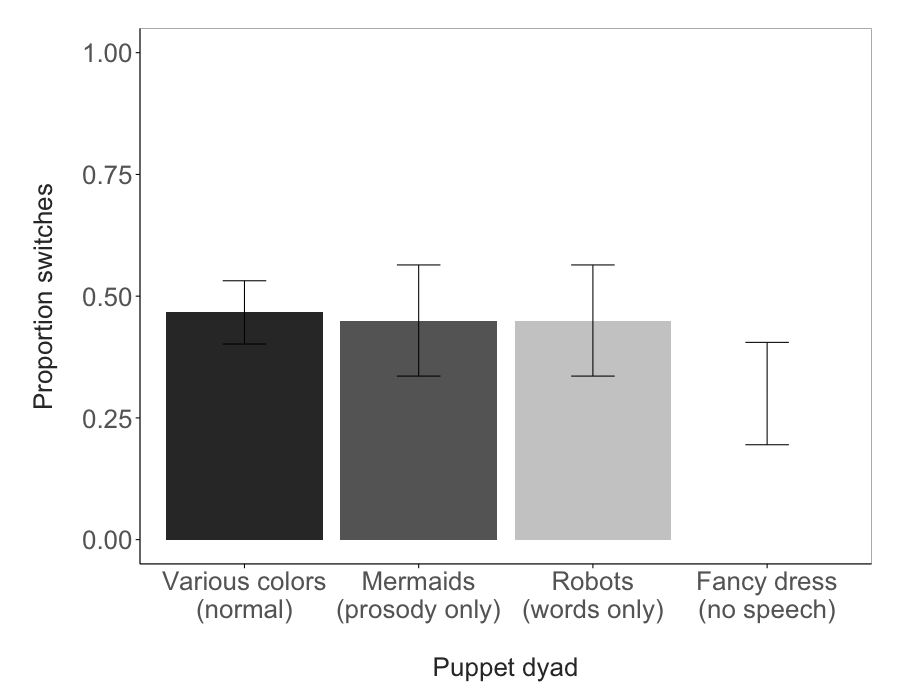
\includegraphics[width=0.95\textwidth]{figures/all-puppetdyads-bars.png}
\end{center}
\caption{Proportion gaze switches across puppet pairs when linguistic condition and conversation are held constant.} 
\label{fig:pairconfound}
\end{figure}

\clearpage

\linespread{1}
\begin{table}
\begin{center}
  \begin{tabular}{llcccc}
%    \hline
           &  Estimate & Std. Error & \textit{z} value & Pr($>$$|$\textit{z}$|$) \\    
    \hline
		 \footnotesize{\textit{Reference level: normal-condition puppets}} &&&& \\
    \hline
     (Intercept) 								& -0.14790	& 0.32796	& -0.451		& 0.652 \\ 
     Puppets$=$\textit{mermaid} 	& -0.07581	& 0.65532	& -0.116		& 0.908 \\ 
     Puppets$=$\textit{robot} 		& -0.07104	& 0.65321	& -0.109		& 0.913 \\ 
     Puppets$=$\textit{party} 		& -0.78206	& 0.68699	& -1.138		& 0.255 \\ 
    \hline
		 \footnotesize{\textit{Reference level: mer-puppets}} &&&& \\
    \hline
     (Intercept) 								& -0.22371	& 0.56832	& -0.394		& 0.694 \\ 
     Puppets$=$\textit{robot} 		& 0.004763	& 0.80096	& 0.006		& 0.995 \\ 
     Puppets$=$\textit{party} 		& -0.70626	& 0.82742	& -0.854		& 0.393 \\ 
    \hline
		 \footnotesize{\textit{Reference level: robot puppets}} &&&& \\
    \hline
     (Intercept) 								& -0.21895	& 0.56565	& -0.387		& 0.699 \\ 
     Puppets$=$\textit{party} 		& -0.71102	& 0.82657	& -0.860		& 0.390 \\ 
    \hline
		 \footnotesize{\textit{Reference level: party-goer puppets}} &&&& \\
    \hline
     (Intercept) 								& -0.9300	& 0.6067		& -1.533		& 0.125 \\ 
  \end{tabular}
\end{center}
  \caption{Model output for children's anticipatory gaze switches with reference levels varied to show all possible pairwise differences between puppet pairs.}
\label{tab:control_exp}
\end{table}
\linespread{2}

In four versions of this model, we systematically varied the reference level of the puppet pair to check for any cross-condition differences. We found no significant effects of puppet pair on switching rate (all \textit{p}$>$0.25; Table \ref{tab:control_exp}).

We take this finding as evidence that our decision to not fully cross puppet pairs and linguistic conditions in Experiment 2 was unlikely to have strongly affected children's anticipatory gaze rates above and beyond the intended effects of linguistic condition.

\end{document}